\documentclass[10pt,a4paper]{article}
\usepackage[utf8]{inputenc}
\usepackage{amsmath}
\usepackage{amsfonts}
\usepackage{amssymb}
\usepackage{amsthm}
\usepackage{float}
\usepackage{mathtools}
\usepackage{geometry}[margin=1in]
\usepackage{xspace}
\usepackage{tikz}
\usepackage{mathrsfs}
\usetikzlibrary{shapes, arrows, decorations.pathmorphing, ducks, automata}
\usepackage[parfill]{parskip}
\usepackage{subcaption}
\usepackage{stmaryrd}
\usepackage{marvosym}
\usepackage{dsfont}
\usepackage{pgfplots}
\usepackage{enumitem}
\usepackage{calc}
\usepackage{tikz-cd}
\usepackage{hyperref}

\hypersetup{
    colorlinks,
    citecolor=black,
    filecolor=black,
    linkcolor=black,
    urlcolor=black
}

\newcommand{\st}{\text{ s.t. }}
\newcommand{\contr}{\lightning}
\newcommand{\im}{\mathfrak{i}}
\newcommand{\R}{\mathbb{R}}
\newcommand{\Q}{\mathbb{Q}}
\newcommand{\C}{\mathbb{C}}
\newcommand{\F}{\mathbb{F}}
\newcommand{\K}{\mathbb{K}}
\newcommand{\N}{\mathbb{N}}
\newcommand{\Z}{\mathbb{Z}}
\renewcommand{\P}{\mathbb{P}}
\renewcommand{\H}{\mathds{H}}
\renewcommand{\O}{\mathcal{O}}
\newcommand{\A}{\mathbb{A}}
\newcommand{\D}{\mathbb{D}}
\newcommand{\nequiv}{\not\equiv}
\newcommand{\powset}{\mathcal{P}}
\renewcommand{\th}[1][th]{\textsuperscript{#1}\xspace}
\newcommand{\from}{\leftarrow}
\newcommand{\legendre}[2]{\left(\frac{#1}{#2}\right)}
\newcommand{\ow}{\text{otherwise}}
\newcommand{\imp}[2]{\underline{\textit{#1.}$\implies$\textit{#2.}}}
\let\oldexists\exists
\let\oldforall\forall
\renewcommand{\exists}{\oldexists\;}
\renewcommand{\forall}{\;\oldforall}
\renewcommand{\hat}{\widehat}
\renewcommand{\tilde}{\widetilde}
\newcommand{\one}{\mathds{1}}
\newcommand{\under}{\backslash}
\newcommand{\injection}{\hookrightarrow}
\newcommand{\surjection}{\twoheadrightarrow}
\newcommand{\jacobi}{\legendre}
\newcommand{\floor}[1]{\lfloor #1 \rfloor}
\newcommand{\ceil}[1]{\lceil #1 \rceil}
\newcommand{\cbrt}[1]{\sqrt[3]{#1}}
\renewcommand{\angle}[1]{\langle #1 \rangle}
\newcommand{\dbangle}[1]{\angle{\angle{#1}}}
\newcommand{\wrt}{\text{ w.r.t. }}

\newcommand*\circled[1]{\tikz[baseline=(char.base)]{
      \node[shape=circle,draw,inner sep=2pt] (char) {#1};}
}

\DeclareMathOperator{\ex}{ex}
\DeclareMathOperator{\id}{id}
\DeclareMathOperator{\upper}{Upper}
\DeclareMathOperator{\dom}{dom}
\DeclareMathOperator{\disc}{disc}
\DeclareMathOperator{\charr}{char}
\DeclareMathOperator{\Image}{im}
\DeclareMathOperator{\ord}{ord}
\DeclareMathOperator{\lcm}{lcm}
\DeclareMathOperator{\aut}{Aut}
\DeclareMathOperator{\diag}{diag}
\DeclareMathOperator{\stab}{stab}
\DeclareMathOperator{\trace}{trace}
\DeclareMathOperator{\ecl}{ecl}
\DeclareMathOperator{\Span}{Span}
\DeclareMathOperator{\Gal}{Gal}
\DeclareMathOperator{\Aut}{Aut}
\DeclareMathOperator{\Frob}{Frob}
\let\div\relax
\DeclareMathOperator{\div}{div}
\DeclareMathOperator{\Div}{Div}
\let\Re\relax
\let\Im\relax
\DeclareMathOperator{\Re}{\mathfrak{Re}}
\DeclareMathOperator{\Im}{\mathfrak{Im}}
\DeclareMathOperator{\Frac}{Frac}
\DeclareMathOperator{\Pic}{Pic}

\let\emph\relax
\DeclareTextFontCommand{\emph}{\bfseries\em}

\newtheorem{theorem}{Theorem}[section]
\newtheorem{lemma}[theorem]{Lemma}
\newtheorem{corollary}[theorem]{Corollary}
\newtheorem{proposition}[theorem]{Proposition}
\newtheorem{conjecture}[theorem]{Conjecture}
\newtheorem{definition}[theorem]{Definition}

\definecolor{burgundy}{rgb}{0.5, 0.0, 0.13}

\tikzset{sketch/.style={decorate,
 decoration={random steps, amplitude=1pt, segment length=5pt},
 line join=round, draw=black!80, very thick, fill=#1
}}


\title{Commutative Algebra}
\begin{document}
\maketitle
\tableofcontents
\newpage
\setcounter{section}{-1}
\section{Introduction}
Commutative Algebra is the study of commutative rings and the spaces on which those rings act, namely modules. It was developed from two key sources: algebraic geometry, and algebraic number theory.

In algebraic geometry we are focused on polynomial rings over a field $k$, whilst in number theory we are focused on $\Z$, the ring of rational integers. Much of this work was done by Grothedieck, but the subject goes back much further, at least to Hilbert who wrote a series of papers on polynomial invariant theory in the late nineteenth century.

As an example, take $\Sigma_n$, the symmetric group on the set $\{1,2,\ldots,n\}$. $\Sigma_n$ acts on $k[x_1, \ldots, x_n]$ by permuting the variables, so that $(\sigma f)(x_1, \ldots, x_n) = f(x_{\sigma^{-1}(1)}, \ldots, x_{\sigma^{-1}(n)})$. $\sigma_n$ acts here via ring automorphisms, and it is then natural to consider the \emph{ring of invariants}, given by $\{f\in k[\mathbf{x}]: \sigma f = f\; \forall \sigma \in \Sigma_n] \coloneqq S$. $S$ is a ring, \emph{the ring of symmetric polynomials}. We can consider the elementary symmetric functions, which are:
\begin{align*}
e_1(x_1, \ldots, x_n) &= x_1 + \ldots + x_n\\
e_2(x_1, \ldots, x_n) &= \sum_{i<j} x_ix_j\\
&\vdots \\
e_n(x_1, \ldots, x_n) &= x_1\ldots x_n
\end{align*}

In fact, $S$ is generated as a ring by these $e_i$, and there are canonical maps $k[y_1, \ldots, y_n] \to S$ such that $Y_i \mapsto e_i$, which is a ring isomorphism.

Hilbert showed that $S$ is finitely generated, and moreover for many other groups, not just symmetric groups.

Along the way, he proved four very deep theorems:
\begin{itemize}
\item Basis theorem
\item Nullstellensatz
\item The polynomial nature of the Hilbert function (leading to the beginnings of dimension theory)
\item The syzygy theorem (leading to the beginnings of homological theory of polynomial rings)
\end{itemize}

In 1921 Emmy Noether extracted the key property that made the basis theorem, namely that a commutative ring is \emph{noetherian} if every ideal is finitely generated (there are several equivalent definitions).

\begin{theorem}[Hilbert's Basis Theorem]
If $R$ is a commutative noetherian ring, then $R[x]$ is also noetherian.
\end{theorem}
\begin{corollary}
If $k$ is a field, then $k[x_1, \ldots, x_n]$ is noetherian.
\end{corollary}

Noether developed a theory of ideals for noetherian rings, for example the existence of primary decomposition, which generalises factorisation into primes in noetherian rings.

\subsection*{Link between Commutative Algebra and Algebraic Geometry}
The starting point for this link is the \emph{fundamental theorem of algebra}, which says that $f \in \C[x]$ is determined up to scalar multiples by its zeros up to multiplicity. Given $f \in \C[x_1, \ldots, x_n]$, there is a polynomial function $\C^n \to \C$ given by $(a_1, \ldots, a_n) \mapsto f(a_1, \ldots, a_n)$.

Different polynomials will yield different functions, and so $\C[x_1, \ldots, x_n]$ can be viewed as a ring of polynomial functions on complex affine n-space.

More specifically, given $I \subseteq \C[x_1, \ldots, x_n]$, we can define the \emph{set of common zeros}, $Z(I) = \{(a_1, \ldots, \_n) \in \C^n : f(a_1, \ldots, a_n) = 0 \; \forall f \in I\}$, called an \emph{(affine) algebraic set}.

\underline{Remarks:}
\begin{itemize}
\item One can replace $I$ by the ideal generated by $I$, and you get the same algebraic set. Similarly, replacing an ideal by a generating set of the ideal leaves the algebraic set. The basis theorem asserts that any algebraic set is the set of common zeros of some \emph{finite} set of polynomials.

\item $\bigcap_j Z(I_j) = Z(\bigcup_j I_j), \bigcup_{j=1}^n Z(i_j) = Z(\prod_{j=1}^n I_j)$, for ideal $I_j$. If we define a topology on $\C^n$ by calling these algebraic sets the closed sets, we get the \emph{Zariski toplogy}, which is a rather coarser topology on $\C^n$ than the usual topology.

\item For $S \subseteq \C^n$, we can define $I(S) = \{f \in \C[x_1, \ldots, x^n] : f(a_1, \ldots, a_n)=0\;\forall (a_1, \ldots, a_n) \in S\}$. This is an \emph{ideal} of $\C[x_1, \ldots, x_n]$, and it is \emph{radical}, i.e. $f^r \in I(s) \implies f \in I(S)$. The Nullstellensatz is a family of results asserting that the correspondence
\begin{align*}
I &\mapsto Z(I)\\
I(S) &\mapsfrom S
\end{align*}
gives a bijection between the radical ideals in $\C[x_1, \ldots, x_n]$ and the algebraic subsets of $\C^n$. In particular, the maximal ideals of $\C[x_1, \ldots, x_n]$ correspond to points in $\C^n$
\end{itemize}

\subsection*{Dimension}
A large portion of the course deals with the dimension of rings. We can define it in three main ways:
\begin{itemize}
\item The maximal length of a chain of prime ideals.
\item In a geometric context in terms of growth rates.
\item The transcendence degree of a field of fractions.
\end{itemize}
For commutative rings, all three give the same answer. There is in fact a fourth method, using homological algebra, which in the case of ``nice''"'' noetherian rings also gives the same answer.

Most of this theory dates back to 1920-1950. Rings of dimension 0 are called \emph{artinian} rings, and in dimension 1 there are special properties which are important in number theory, particularly in the study of algebraic curves.

\section{Noetherian Rings: Definitions and Examples}
Throughout this section, $R$ is a commutative ring with a 1.

\begin{lemma}
Let $M$ be a (left) $R$-module. The following are equivalent:
\begin{enumerate}
\item All submodules of $M$ (including $M$ itself) are finitely generated.
\item The ascending chain condition (ACC) holds: there are no strictly increasing infinite chains of submodules.
\item The maximum condition of submodules holds: any nonempty set $S$ of submodules of $M$ has a maximal element $L$, i.e. $L \subseteq L', L' \in S \implies L = L'$.
\end{enumerate}
\end{lemma}
\begin{proof}\hspace*{0cm}\\
\imp{1}{2} Suppose there is a strictly increasing chain $N_1 \subsetneq N_2 \subsetneq \ldots$, and let $N = \bigcup_{i=1}^\infty N_i$. By \textit{1} $N$ is finitely generated, say by $m_1, \ldots, m_r$. Each $m_i$ lies in some $N_{n_i}$. Then let $n = \max_i n_i$, so that $m_i \in N_n$. Then $N_n = M$, contradicting strict ascent.

\imp{2}{3} Assume ACC. Pick $M_1 \in S$. If it is the maximal member then we're done. If not, there is $M_2 \supsetneq M_1$. If $M_2$ is maximal, then we're done, otherwise there is some $M_3 \supsetneq M_2$, and so on. By ACC this process terminates, and we get a maximal element.

\imp{3}{1} Let $N \triangleleft M$, and let $S$ be the collection of all finitely generated submodules of $N$. Then $S \neq \emptyset$ since it contains the 0 submodule. So $S$ contains a maximal member, say $L$. We then claim $N = L$. If $x \in N$ then $L+Rx \in S$, and by maximality of $L$, $x \in L$.
\end{proof}

\begin{definition}
An $R$-module satisfying \textit{1, 2, 3} is \emph{noetherian}.
\end{definition}

\begin{lemma}
Let $N \triangleleft M$. Then $M$ is noetherian if and only if $N$ and $M/N$ are noetherian.
\end{lemma}
\begin{proof}\hspace*{0cm}\\
\underline{$\implies$} Let $M$ be noetherian, so that all its submodules are finitely generated. This property is inherited by $N$. Also, the submodules of $M/N$ are all of the form $Q/N$ with $Q \triangleleft M$ containing $N$. If $M$ is noetherian, then $Q$ is finitely generated, say by $x_1, \ldots, x_r$. Then $x_1 + N, \ldots, x_r+ N$ generates $Q/N$.

\underline{$\impliedby$} Let $N, M/N$ be noetherian, and let $L_1 \subset L_2 \subset L_3 \subset \ldots$ be a strictly increasing chain of submodules of $M$. Set $Q_i / N = (L_i + N)/N$, and $N_i = L_i \cap N$. These give ascending chains of submodules of $M/N$ and $N$ respectively. By ACC there are $r, s$ with $Q_i/N = Q_r/N$ for $i\geq r$, $N_i = N_s$ for $i\geq s$. Let $k = \max\{r, s\}$. Then we claim $L_i = L_k$ for $i \geq k$. Pick $\ell \in L_i$, $i \geq k$. Then $\ell + N \in Q_k/N$, and so there is some $\ell' \in L_k$ such that $\ell-\ell' \in N \cap L_i = N\cap L_k$. So $\ell \in L_k$, and the claim is proved. Hence our original ascending chain was not strictly increasing, $\contr$.
\end{proof}
\begin{lemma}
\begin{enumerate}
\item If $M, N$ are $R$-modules, then $M \oplus N$ is noetherian iff $M$ and $N$ are noetherian.
\item If $M_1, \ldots, M_n$ are $R$-modules then $M_1 \oplus \ldots \oplus M_n$ is noetherian iff each $M_i$ is noetherian.
\item If $M$ is noetherian then every homomorphic image of $M$ is noetherian.
\item Suppose $M$ can be expressed as a sum of finitely many submodules (not necessarily as a direct sum) $M = M_1 + \ldots + M_n$. Then $M$ is noetherian iff each $M_i$ is.
\end{enumerate}
\end{lemma}
\begin{proof}
\begin{enumerate}
\item $M \cong N/N$, so this follows by \textbf{1.3}.
\item Apply \textit{1} and induction on $n$.
\item If $\theta: M \to N$ then $\Image \theta \cong M/\ker\theta$, so apply \textbf{1.3}.
\item The forwards direction follows as $M_i \triangleleft M$. For the reverse, there is a map from $M_1 \oplus \ldots \oplus M_n \to M$, $(m_1, \ldots, m_n) \mapsto m_1+\ldots+m_n$, and then apply \textit{2} and \textit{3}.
\end{enumerate}
\end{proof}

\begin{definition}
A ring $R$ is \emph{noetherian} if it is noetherian as a (left) $R$-module
\end{definition}

\underline{Remark:}  Submodules of $R$ as an $R$-module are the same as ideals of $R$ as a ring, and so the ACC for modules gives us the ACC for ideals.

\begin{lemma}
Let $R$ be a noetherian ring. Then any finitely generated $R$-module $M$ is noetherian.
\end{lemma}
\begin{proof}
  Suppose $M = Rm_1 + \ldots + Rm_n$. There exist $R$-module epimorphisms:
  \begin{align*}
    R &\to Rm_i\\
    r &\mapsto rm_i
  \end{align*}
  $R$ is noetherian, so $Rm_i$ is as the homomorphic image of $R$. Then, by \textbf{1.4} \textit{(4)}, so is $M$.
\end{proof}
\begin{theorem}[Hilbert Basis Theorem]
  Let $R$ be a noetherian ring. Then the polynomial ring $R[x]$ is noetherian.
\end{theorem}
\begin{proof}
  We show that every ideal of $R[x]$ is finitely generated. Let $I$ be an ideal. We define $I(n) = \{f \in I: \deg f \leq n\}$. Then $I(n) \neq \emptyset$ as $0 \in I(n)$, and $I(0) \subseteq I(1) \subseteq I(2) \subseteq \ldots$.

  Let $R(n) = \{\text{Coefficient of $x^n$ in $f$} : f \in I(n)\} \subseteq R$. We claim $R(n) \triangleleft R$, and $R(n) \subseteq R(n+1)$.

  To see this, suppose $a, b \in R(n)$. Then there are polynomials $f(x) = ax^n + \ldots, g(x) = bx^n + \ldots$ in $I$, where $\ldots$ indicates lower order terms. Since $I \triangleleft R$, $f\pm g \in I$, $rf \in I$ for all $r \in R$, and $xf \in I$.

  Hence $a \pm b \in R(n), ra \in R(n)$, and $a \in R(n+1)$, and the claim is proved.

  So then we have a chain $R(0) \subseteq R(1) \subseteq R(2) \subseteq \ldots$ terminates, so we may say $R(n) = R(N)\forall n \geq N$. Each of $R(0), \ldots, R(N)$ is a finitely generated ideal of $R$, say $R(j) = (a_{j,i}, \ldots, a_{j, k_j})$.

  Then by definition of $R(j)$, we may take polynomials $f_{j,1}, \ldots, f_{j, k_j}$ in $I(j)$ which have the $a_{j,i}$ as their leading coefficients.

  Clearly $I \supseteq (f_{j, k} : 0 \leq j \leq N, 1 \leq k \leq k_j) \eqqcolon J$ - it remains to show that equality holds, then we will have found a finite generating set of $I$. So pick $f \in I$, then we claim $f \in J$, and prove this by induction on the degree of $f$.

  If $\deg f = 0$, then $f(x) = a$, say. But then $a \in R(0)$, and so $a = \sum_i r_i a_{0, i}$ for some $r_i \in R$. Since $f_{0, i}$ has $a_{0, i}$ as its leading coefficient and has degree zero, $f_{0, i}(x) = a_{0, i}$, and $f = \sum_i r_i f_{0,i} \in J$.

  If instead $\deg f = n$, with $0 < n \leq N$, and the claim holds for all $g$ with $\deg g < n$, then write $f(x) = ax^n + \ldots$. $a \in R(n)$ then by definition, so $a= \sum_i r_{n, i} a_{n,i}$ for some $r_{n,i} \in R$.
  Then define $g(x) = f(x) - \sum_i r_{n, i} f_{n, i}(x)$. $g(x)$ has degree $\leq n$, and the coefficient of $x^n$ is $a - a = 0$, hence $\deg g < n$. Since $f_{n, i} \in I$, we have $g \in I$, and hence by induction $g \in J$. But $f_{n, i} \in J$ as well, so $f \in J$.

  Finally if $\deg f = n$, with $n > N$, and the claim holds for all $g$ with $\deg g <n$, again write $f(x) = ax^n + \ldots$. Then $a \in R(n) = R(N)$, so $a = \sum r_{N, j} a_{N,j}$ for $r_{N,j} \in R$. We may then define $g(x) = f(x) - \sum_i x^{n-N} r_{N, j} f_{N, j}(x)$, and use the same argument as in the previous paragraph to deduce that $f \in J$.

  Hence $I \subseteq J$, and so $I = J$ and $I$ is finitely generated. But $I$ was an arbitrary ideal of $R[x]$, so $R[x]$ is noetherian.
\end{proof}

In practice, one uses \emph{Gr\"obner bases} for ideals - these are generating sets with extra properties that make algorithms more efficient.

\underline{Examples:}
\begin{itemize}
  \item Fields are noetherian.
  \item Principle Ideal Domains (PIDs) are noetherian.
  \item $\{q \in Q : q = \frac{m}{n}, m, n \in \Z, p \nmid n \text{ for some fixed prime } p\}$, an example of a \textit{localisation} of $\Z$. All localisations of noetherian rings are noetherian - we will see this later.
  \item $k[x_1, x_2, \ldots]$ is not noetherian: $(x_1) \subsetneq (x_1, x_2) \subsetneq$ is an infinite strictly increasing chain.
  \item $k[x_1, x_2, \ldots, x_n]$ is noetherian - this follows by induction using the Hilbert basis theorem.
  \item $\Z[x_1, x_2, \ldots, x_n]$ is noetherian, so any finitely generated commutative ring is noetherian: if $R$ is generated by $r_1, \ldots, r_n$, then there is an epimorphism $\Z[x_1, \ldots, x_n] \to R$ given by $x_i \mapsto r_i$, and $R$ is the homomorphic image of a noetherian ring.
  \item If $A$ is a free abelian group, write $\Z A$ for its group algebra, which is the set of formal linear combinations of elements of $A$, i.e. terms of the form $\sum_{\alpha \in A} \lambda_\alpha \alpha$ where $\lambda_\alpha \in \Z$ and only finitely many of the $\lambda_\alpha$ are nonzero.

  If $A$ is generated as a group by $g_1, \ldots, g_n$, then its group algebra is generated as a ring by $g_1, g_1^{-1}, \ldots, g_n, g_n^{-1}$.
  \item $k[[x]]$, the ring of formal power series with coefficients in $k$, is noetherian.
\end{itemize}
There are also some non-commutative examples that are both left and right noetherian:
\begin{itemize}
  \item Enveloping algebras of a finite dimensional Lie algebra.
  \item Iwasawa algebras of compact $p$-adic groups.
\end{itemize}

\begin{theorem}
  If $R$ is noetherian, then $R[[x]]$ is noetherian.
\end{theorem}
\begin{proof}[Proof 1]
  As in \textbf{1.7}, consider $R(n) =$ the set of trailing coefficients $a_n$, for elements $a_nx^n +$ higher order terms, and mimic the proof. This is on example sheet 1.
\end{proof}
We will give a second proof, which uses
\begin{theorem}[Cohen's Theorem]
  If every prime ideal in a ring $R$ is finitely generated, then $R$ is noetherian.
\end{theorem}
\begin{proof}
  If $R$ is not noetherian, then there is a family of non-finitely generated ideals. Call it $\mathscr{S}$. By assumption, $\mathscr{S} \neq \emptyset$. Partially order $\mathscr{S}$ by inclusion.

  Suppose $I_1 \subseteq I_2 \subseteq \ldots$ is a chain of non-finitely generated ideals. Then we claim $\bigcup_i I_i$ is also non-finitely generated.

  If it were, say by $(a_1, \ldots, a_k)$, then $a_i \in I_{n(i)}$ for some finite integer $n(i)$, and so, if $N = max \{n(i) : 1\leq i \leq k\}$, $N$ is also finite and $a_i \in I_N$ for all $i$. But then $I_N = I_n$ for all $n \geq N$, and in particular $I_N$ is finitely generated $\contr$.

  So $\mathscr{S}$ has upper bounds to its chains, and so we may apply Zorn's lemma to get a maximal element of $\mathscr{S}$, say $I$, so that $I$ is not finitely generated but any ideal containing $I$ is finitely generated.

  We now claim $I$ must be prime. Suppose $a \notin I, b \notin I$, but $ab \in I$. Then $I + (a) \supsetneq I$, so $I + (a)$ is finitely generated, say by $i_1 + r_1a, \ldots, i_n + r_na$. Define $J = \{s \in R : sa \in I\} \supseteq I+(b)\supsetneq I$. Again, $J$ is finitely generated.

  Take $t \in I \subset I+(a)$, so $t = u_1(i_1+r_1a) + \ldots + u_n(i_n+r_n a)$ for some $u_i \in R$. So $t = u_1i_1 + \ldots +u_ni_n + (u_1r_1 + \ldots +u_nr_n)a \in (i_1) + (i_2) + \ldots + (i_n) + Ja$.

  Hence $I \subseteq (i_1) + \ldots + (i_n) + Ja$, so $I = (i_1) + \ldots + (i_n) + Ja$, so $I$ is finitely generated $\contr.$

  So $I$ must be prime, but then by our hypothesis $I$ is still finitely generated $\contr$. So $R$ must be noetherian.
\end{proof}
We will also use the following lemma:
\begin{lemma}
  Let $P$ be a prime ideal of $R[[x]]$ and $\theta : R[[x]] \to R$, $x \mapsto 0$. Then $P$ is finitely generated if and only if $\theta(P)$ is a finitely generated ideal of $R$.
\end{lemma}
\begin{proof}
  Clearly if $P$ is finitely generated then $\theta(P)$ is.

  Conversely, suppose $\theta(P) = Ra_1 + \ldots + Ra_n$.

  If $x \in P$, then $P = (a_1, \ldots, a_n, x)$.

  This is immediate - if $g \in P$, $g = a + $ higher order terms. Now $a \in (a_1, \ldots, a_n)$, so $g = \sum_i r_i a_i + xg'$ as required.

  If $x \notin P$, then let $f_1, \ldots, f_n$ be power series with constant terms $a_1, \ldots, a_n$ respectively. Then $P = (f_1, \ldots, f_n)$.

  Take $g \in p$, say $g = b +$ higher terms, with $b$ the constant term. Then $b = \sum b_i a_i$, so $g - \sum b_i f_i = g_1 x$ for some $g_1$. Note that $g_1 x \in P$, $P$ is prime, and $x \notin P$, so $g_1 \in P$. Similarly, $g_1 = \sum c_i f_i + g_2 x$, and $g_2 \in P$. Continuing, we get $h_1, \ldots, h_n \in R[[x]]$, where $h_i = b_i + c_i x + \ldots$ with $g = h_1f_1 + \ldots + h_nf_n$.
\end{proof}

We are now ready to give the second proof the $R$ noetherian implies $R[[x]]$ noetherian:
\begin{proof}[Proof 2]
  Suppose $P$ is a prime ideal of $R[[x]]$. Then $P$ is finitely generated iff $\theta(P)$ is. But $R$ is noetherian, so $\theta(P)$ is finitely generated, so $P$ was finitely generated. Then we apply Cohen's theorem to get $R[[x]]$ noetherian.
\end{proof}

\subsection{Ideal Structure}
Here, we assume $R$ is a commutative ring with a 1, not necessarily noetherian.
\begin{lemma}
  The set $N(R)$ of all nilpotent\footnote{An element $x$ of a ring is called nilpotent if there is some integer $m$ such that $x^m = 0$.} elements of $R$ is an ideal, and $R/N(R)$ has no nonzero nilpotent elements.
\end{lemma}
\begin{proof}
  If $x \in N(R)$, then $x^m = 0$ for some $m$. Hence $(rx)^m = 0$ for all $r \in R$, and so $rx \in N(R)$.

  If $x, y \in N(R)$, then $x^n = 0, y^m = 0$ for some $n, m$. Then $(x+y)^{n+m-1}$ expands to give terms $\lambda x^s y^t$ where $s+t = m+n-1$. So either $s \geq n$ or $y \geq m$, so all the terms are zero, and $x+y \in N(R)$.

  So $N(R) \triangleleft R$.

  Finally, if $s \in R/N(R)$ then $s = x+N(R)$. Note that $s^n = x^n + N(R)$ for all $n$. If $x + N(R)$ is nilpotent then $(x+N(R))^m = N(R)$ for some $m$, and hence $x^m \in N(R)$. So $x^m$ is nilpotent, and $(x^m)^n = x^{mn} = 0$ for some $n$. But then $x$ is nilpotent, so $x+ N(R) = 0 + N(R)$.
\end{proof}
\begin{definition}
  $N(R)$ is called the \emph{nilradical} of $R$.
\end{definition}

\begin{theorem}[Krull]
  $N(R)$ is the intersection of all prime ideals of $R$.
\end{theorem}
\begin{proof}
  Let $I = \bigcap_{P\text{ prime}} P$. If $x \in R$ is nilpotent then $x^n = 0 \in P \forall P$. So $x \in P \forall P \implies x \in I$, so $N(R) \subseteq I$.

  Suppose $x$ is not nilpotent. Let $\mathscr{S}$ be the family of ideals $J$ such that for $n > 0$, $x^n \notin J$. Then $(0) \in \mathscr{S}$, so $\mathscr{S} \neq \emptyset$, and a union of a chain of ideals in $\mathscr{S}$ is also in $\mathscr{S}$. We apply Zorn's lemma to get a maximal element $J_1$.

  We claim $J_1$ is prime - suppose $yz \in J_1$, but $y, z \notin J_1$. So the ideals $J_1 + Ry, J_1 + Rz$ strictly contain $J_1$, and so $x^m  \in J_1+Ry$ and $x^n  \in J_1 + Rz$. But then $x^{m+n} \in J_1 + Ryz = J_1 \contr.$

  So $J_1$ is prime, so contains $I$, and hence $x \notin I$, so $I \supseteq N(R)$. Thus $I = N(R)$.
\end{proof}

\begin{definition}
  The \emph{radical} $\sqrt{I}$ of an ideal $I$ is defined by $\{r \in R : \exists k \in \N \st r^k \in I\}$.
\end{definition}
Note that $\sqrt{I}/I = N(R/I)$, and $\sqrt{I} = \bigcap\limits_{\text{prime  }P \supset I} P$. We say an ideal $I$ is radical if $I = \sqrt{I}$

\begin{definition}
  The \emph{Jacobson radical} $J(R)$ of $R$ is the intersection of all the maximal ideals of $R$ (so $N(R) \subseteq J(R)$).
\end{definition}

\begin{theorem}[Nakayama's Lemma]
  If $M$ is a finitely generated $R$-module with $MJ = M$, where $J = J(R)$, then $M = 0$.
\end{theorem}
\begin{proof}\footnote{Note - this is not the usual Atiyah-Macdonald proof, but this one can be adapted to the case of non-commutative rings.}
  If $M \neq 0$ and is a finitely generated $R$-module, then by Zorn's lemma there are maximal proper submodules.

  Take $M_1$ maximal in $M$. Then $M/M_1$ is irreducible (or simple), hence generated by $m+M_1$ say.

  Then, considering the map $R \to M/M_1; r\mapsto rm+M_1$, which is an $R$-module homomorphism with kernel a maximal ideal, we see that $M/M_1 \cong R/I$, where $I$ is a maximal ideal of $R$, so $MI \leq M_1$

  Finally, $J \leq I$, then $MJ \leq MI \leq M_1 \lneq M$, so if $M \neq 0, MJ \lneq M$.
\end{proof}


For a commutative ring $R$, $N(R) \leq J(R)$. These need not be equal - for example, take $R = \left\{\frac{m}{n} \in \Q: p \nmid n\right\} = \Z_{(p)}$. This has unique maximal ideal $P = \left\{\frac{m}{n} \in \Q : p|m, p \nmid n \right\}$. It is an integral domain, so has no nonzero nilpotent elements, so $N(R) = (0)$, and $J(R) = P$.

For rings $R = k[x_1, \ldots, x_n]/I$ with $k$ algebraically closed and $I$ any ideal, we do have $N(R) = J(R)$ - this is the Nullstellensatz - see later on.

\underline{Example:} A commutative ring is \emph{artinian} if it doesn't contain an infinite strictly descending chain of ideals (or equivalently if every nonempty set of ideals has a minimal member). An $R$-module is \emph{artinian} if it satisfies the analogous properties for submodules. As an exercise (on the first example sheet), prove that artinian rings are noetherian.

For example, $\Z/p\Z, k[x]/(f)$. $k[x]$ is not artinian ($(x) >(x^2) > \ldots)$).

Recall that $I$ is prime if and only if one following three equivalent properties holds:
\begin{align*}
  ab \in I \implies a \in I \text{ or } b \in I\\
  R/I \text{ is an integral domain}\\
  I_1I_2 \subseteq I \implies I_1 \subseteq I \text{ or }I_2 \subseteq I
\end{align*}
\underline{Claim:} $J(R) = N(R)$ for artinian rings $R$\\
This follows if we can show that $R$ artinian $\implies$ every prime ideal is maximal.
\begin{proof}
  Let $P$ be prime, $x \notin P$. By the descending chain condition, $(x) \supseteq (x^2) \subseteq \ldots$ is not strict, so $(x^n) = (x^{n+1}) = \ldots$ for some $n$. Hence $x^n = yx^{n+1}$ for some $y$. Then $x^n(1-xy) = 0 \in P$. But $x^n \notin P$, and $P$ is prime, so $1-xy \in P$. Thus $y+P$ is the inverse of $x+P$ in $R/P$, and so $R/P$ is a field, and $P$ is maximal.
\end{proof}

\begin{lemma}[Artin-Tate]
  Suppose we have commutative rings $R \leq S \leq T$. Suppose $R$ is noetherian and $T$ is generated as a ring by $R$ and finitely many elements $t_1, \ldots, t_n$. Suppose that $T$ is a finitely generated $S$-module. Then $S$ is generated by $R$ and finitely many elements as an $R$-algebra.
\end{lemma}
\begin{proof}
  $T$ is generated by $x_1 \ldots, x_m \in T$ as an $S$-module, so $T = Sx_1 + \ldots + Sx_m$. Then:
  \begin{align*}
    t_i &= \sum_j s_{ij}x_j,\;\;\; s_{ij} \in S \tag{1}\\
    x_ix_j &= \sum_k s_{ijk} x_k, \;\;\; s_{ijk} \in S\tag{2}
  \end{align*}
  Let $S_0$ be the ring generated by $R$, the $s_{ij}$ and the $s_{ijk}$, so that $R \leq s_0 \leq S$.

  Any element of $T$ is polynomial in the $t_i$ with coefficients in $R$. In (1), (2), each element is a linear combination of the $x_j$ with coefficients in $S_0$. Thus $T$ is a finitely generated $S_0$-module. But $S_0$ is noetherian, being generated as a ring by $R$ and finitely many elements. $T$ is noetherian as an $S_0$-module, and $S$ is an $S_0$-submodule of $T$, hence is finitely generated as an $S_0$-module.

  But $S_0$ is generated by $R$ and finitely many elements, so $S$ is generated by $R$ and finitely many elements.
\end{proof}
\begin{lemma}[Zariski]
  Let $k$ be a field, and $R$ a finitely generated $k$-algebra. If $R$ itself is a field, then it is a finite algebraic extension of $k$, i.e. a finitely generated $k$-space.
\end{lemma}
\begin{proof}
  Suppose $R$ is generated by $k$ and $x_1, \ldots, x_n$, and is a field. If $R$ is not a finite algebraic extension over $k$, then we can reorder the $x_1, \ldots, x_n$ so that $x_1, \ldots, x_m$ are algebraically independent, i.e. the ring generated by $k$ and $x_1, \ldots, x_m$ is a polynomial algebra $k[x_1, \ldots, x_m]$, and $x_{m+1},\ldots, x_n$ are algebraic over the field of fractions $F = k(x_1, \ldots, x_m)$. Because $R$ is not finite algebraic over $k$, $m\geq 1$.

  Hence $R$ is a finite algebraic extension over $F$, and $R$ is a finitely generated $F$-module, (i.e. vector space). Apply Artin-Tate (\textbf{1.17}) for $k \leq F \leq R$, it follows that $F$ is a finitely generated $k$-algebra by $k$ and $q_1 \ldots, q_t$ say, with each $q_i =f_i/g_i$, where $f_i, g_i \in k[x_1, \ldots, x_m], g_i \neq 0$.

  Now there is a polynomial $h$ which is prime to each of the $g_i$s, e.g. $g_1\ldots g_m + 1$, and the element $1/h$ cannot be in the ring generated by $k$ and $q_1, \ldots, q_t$. This a contradiction, and hence $m=0$, and $R$ was indeed algebraic over $k$.
\end{proof}
\begin{theorem}[Weak Nullstellensatz]
  Let $k$ be a field, $T$ a finitely generated $k$-algebra. Let $P$ be a maximal ideal of $T$. Then $T/P$ is a finite algebraic extension of $k$. In particular, if $k$ is algebraically closed and $T$ is the polynomial algebra, then the maximal ideals are of the form $(x_1-a_1, \ldots, x_n-a_n)$.
\end{theorem}
\begin{proof}
  See later.
\end{proof}
\begin{theorem}[Strong Nullstellensatz]
  Let $k$ be an algebraically closed field, and $R$ a finitely generated $k$-algebra. Then $N(R) = J(R)$. Thus, if $I$ is a radical ideal of $k[x_1, \ldots, x_n]$ and $R = k[x_1, \ldots, x_n]/I$, then the intersection of the maximal ideals of $R$ is 0.

  Furthermore, any radical ideal is the intersection of the maximal ideals containing it.
\end{theorem}
\begin{proof}
  Deferred until chapter 2.
\end{proof}
\begin{proof}[Proof of \textbf{1.19}]
  Let $P$ be the maximal ideal of the finitely generated $k$-algebra $T$. Put $R = T/P$. By Zariski's lemma, $T/P$ over $k$  is a finite algebraic extension. If $k$ is closed, then $k = T/P$. Set $\pi:T \to k$ with kernel $P$.

  We then claim that $\ker \pi = (x_1 - \pi(x_1), \ldots, x_n - \pi(x_n))$.

  Now $\pi$ fixes elements of $k$, so the RHS is in the kernel. Conversely, $T/(x_1-\pi(x_1), \ldots, x_n-\pi(x_n))$ is a 1-dimensional $k$-space, so the kernel is contained in the RHS, and so they are equal.

  Recall the bijection proposed earlier between radical ideals in $\C[\mathbf{x}]$ and affine algebraic sets in $\C^n$.

  Rephrase this by defining $Q_{(a_1, \ldots, a_n)} = (x_1-a_1, \ldots, x_n-a_n)$. We claim there is a bijection:

  \begin{align*}
    \{\text{radical ideals}\} &\leftrightarrow \{\text{algebraic subsets}\}\\
    I &\mapsto \{(a_1, \ldots, a_n) : I \subseteq Q_{(a_1, \ldots, a_n)}\}\\
    \bigcap_{(a_1, \ldots, a_n) \in S}Q_{(a_1, \ldots, a_n)} &\mapsfrom S
  \end{align*}
\end{proof}

\subsection{Minimal and Associated Primes}
\begin{lemma}
  If $R$ is noetherian, then any ideal $I$ contains a power of its radical $\sqrt{I}$. In particular, $N(R)$ is nilpotent, i.e. $N(R)^m = (0)$ for some $m$, as $N(R) = \sqrt{(0)}$.
\end{lemma}
\begin{proof}
  Suppose $x_1, \ldots, x_m \in \sqrt{I}$ generate $\sqrt{I}$ as an ideal. Then $x_i^{n_i} \in I$ for some $n_i$. Then, if $n$ is sufficiently sufficiently large (e.g. $n \geq \sum (n_i-1) + 1$). Then $\sqrt{I}^n$ is generated by $x_1^{r_1}, \ldots, x_m^{r_m}$ with $\sum r_i = n$. We must thus have some $r_i \geq n_i$, and so $\sqrt{I}^n \subseteq I$.
\end{proof}

\begin{lemma}
  If $R$ is noetherian, then a radical ideal is the intersection of finitely many prime ideals.
\end{lemma}
\begin{proof}
  Suppose not for contradiction, and take a maximal element $I$ from the set of radical ideals not of this form (using Zorn's lemma). We then claim that $I$ is prime, yielding a contradiction.

  If not, there is $J_1, J_1 \nsubseteq I$ with $J_1J_2 \subseteq I$. If necessary, replace $J_i$ by $J_i + I$, we can assume $I \subsetneq J_1, J_2$.

  Then by the maximality of $I$, $\sqrt{J_1} = Q_1 \cap \ldots Q_m$; $\sqrt{J_2} = Q_1'\cap\ldots\cap Q_n'$ as prime intersections.

  Set $J = \sqrt{J_1} \cap \sqrt{J_2} = Q_1 \cap\ldots\cap Q_m\cap Q_1'\cap\ldots\cap Q_n'$. So $J^{n_1} \leq J_1, J^{n_2} \leq J_2$ for some $n_1, n_2$. Hence $J^{n_1+n_2} \leq J_1J_2\leq I$. But $I$ is radical, so $J \leq I$. Now all $Q_i, Q_j'$ contain $I$, so $J \geq I$. Thus $J=I \contr$.
\end{proof}

Now suppose by the previous lemma that any radical ideal $\sqrt{I} = P_1\cap\ldots\cap P_m$ is an intersection of finitely many primes. We can remove $P_i$ from the list if it contains any of the others, so \textsc{wlog} we may assume that $P_i \nleq P_j$ for any $i \neq j$. If $P$ is prime with $\sqrt{I} \leq P$, then $P_1 \ldots P_m \leq \bigcap_i P_i = \sqrt{I} \leq P$, and so some $P_i \leq P$.

\begin{definition}
  The \emph{minimal primes P over an ideal I} of a noetherian ring are those such that, if $P'$ is prime with $I \leq P' \leq P$, then $P' = P$.
\end{definition}
Clearly the $P_i$ mentioned above are minimal primes over $I$. In fact:

\begin{lemma}
  Let $I$ be an ideal in a noetherian ring. Then $\sqrt{I}$ is the intersection of the minimal primes over $I$, and $I$ contains a finite product of the minimal primes over $I$.
\end{lemma}
\begin{proof}
  Each minimal prime over $I$ contains $\sqrt{I}$. So the primes minimal over $I$ are precisely the minimal ones over $\sqrt{I}$. We know $\sqrt{I}$ is the intersection of these, and thus their product lies in $\sqrt{I}$, and \textbf{1.21} gives the last part.
\end{proof}

\underline{Example:} The Nullstellensatz bijection between radical ideals of $\C[x_1, \ldots, x_n]$ and algebraic subsets of $\C^n$.

Suppose $(a_1, \ldots, a_n)$ is a common zero of all $f\in I$, a radical ideal. Then $I \leq (x_1-a_1, \ldots, x_n-a_n)$. This latter ideal is maximal as it is the kernel of $\C[x_1, \ldots, x_n] \to \C; x_i \mapsto a_i$.

Now consider
\[\bigcap\limits_{\substack{(a_1, \ldots, a_n)\\\text{common zeros}\\\text{of all }f\in I}}(x_1-a_1, \ldots, x_n-a_n)\]

This ideal is radical, and the bijection in the Nullstellensatz implies that this radical ideal is the same as $I$. Thus $I$ is an intersection of maximal ideals, and moreover all maximal ideals are of the form $(x_1-a_1, \ldots, x_n-a_n)$. Also, for any ideal $J_1$ of $\C[x_1, \ldots, x_n]$, we have $N(\C[x_1, \ldots, x_n]/J_1) = J(\C[x_1, \ldots, x_n]/J_1)$.

\subsection{Annihilators and Associated Primes}
\begin{definition}
  Let $M$ be a finitely generated $R$-module, where $R$ is noetherian. The \emph{annihilator} of $m$, $\ann(m) = \{r \in R: rm=0\}$. A prime ideal $P$ is an \emph{associated prime} of $M$ if it is the annihilator of an element of $M$

  We call the set of associated primes $\Ass(M)$.
\end{definition}
For example, $\Ass(R/P) = \{P\}$ for $P$ prime.

\begin{definition}
  A submodule $N$ of $M$ is \emph{p-primary} (or just \emph{primary}) if $\Ass(M/N) = \{p\}$ for a prime ideal $p$. An ideal is \emph{p-primary} if $I$ is p-primary as a submodule of $R$.
\end{definition}
\begin{lemma}
  If $\ann(M) = P$ for a prime ideal $P$, then $P \in \Ass(M)$.
\end{lemma}
\begin{proof}
  Suppose that $M$ is generated by $m_1, \ldots, m_k$. Let $I_j = \ann(m_j)$. Then the product $\prod I_j$ annihilates each $m_j$, so $\Pi I_j \leq \ann(M) = P$. So $I_j = P$ for some $j$ as $P$ prime, and so $P \in \Ass(M)$.
\end{proof}
\begin{lemma}
  Let $Q$ be maximal amongst all annihilators of nonzero elements. Then $Q$ is a prime ideal and so $Q \in \Ass(M)$.
\end{lemma}
\begin{proof}
  Let $Q = \ann(m)$ and $r_1r_2 \in \Q, r_2 \notin \Q$. We show that $r_1 \in Q$.

  Now $r_1r_2 \in Q \implies r_1r_2m = 0$, so $r_1 \in \ann(r_2m)$.

  And $r_2 \notin Q \implies r_2m\neq 0$. But $Q \leq \ann(r_2m)$, and hence $Q$ and $r_2$ lie in $\ann(r_2m)$. By maximality, $Q = \ann(r_2m)$, and so $r_1 \in Q$.
\end{proof}
\begin{lemma}
  For finitely generated nonzero $R$-module $M$, where $R$ is noetherian, there is a chain
  \[ 0\lneq M_1 \lneq M_2 \lneq \ldots \lneq M_t = M\]
  of submodules with $M_i/M_{i-1} \cong R/P_i$ for some prime ideal $P_i$.
\end{lemma}
\begin{proof}
  By \textbf{1.28}, there is $0\neq m_1 \in M$ with $\ann(m_1)$ prime, say $P_1$. Set $M_1 = Rm_1$. Hence $M_1 \cong R/P_1$. Repeat for $M/M_1$ to find $M_2/M_1 \cong R/P_2$ for some prime $P_2$. Continue - the noetherian property forces the process to terminate.
\end{proof}
\begin{lemma}
  $N \subseteq M \implies \Ass(M) \subseteq \Ass(N) \cup \Ass(M/N)$.
\end{lemma}
\begin{proof}
  Take $P \in \Ass(M)$, so that $P = \ann(m)$ for some $m \in M$, and $P$ is prime.

  Let $M_1 = Rm = R/P$. For any $0 \neq m_1 \in M_1$, we have $\ann(m_1) = P$, since $P$ is prime. If $M_1 \cap N \neq 0$, then there is $x \in M_1 \cap N$ with $\ann(x) = P$, and so $P \in \Ass(N)$. Otherwise, $M_1 \cap N = 0$, and the image of $M_1$ in $M/N$ is isomorphic to $R/P$, and hence $P \in \Ass(M/N)$.
\end{proof}
\begin{lemma}
  $\Ass(M)$ is finite for any finitely generated $R$-module, where $R$ is noetherian.
\end{lemma}
\begin{proof}
  Apply \textbf{1.30} inductively to the chain in \textbf{1.29} recalling that $\Ass(R/P_i) = \{P_i\}$. We thus conclude $\Ass(M) \subset \{P_1, \ldots, P_t\}$ is finite.
\end{proof}
\begin{proposition}
  Each minimal prime over an ideal $I$ is an associated prime, i.e.:
  \[\{\text{minimal primes over }I\} \subseteq \Ass(R/I)\]
\end{proposition}
\begin{proof}
  By \textbf{1.24}, there is a product of minimal primes over $I$, possibly with repetitions, contained in $I$, say $p_1^{s_1}\ldots p_n^{s_n} \leq I$ with $p_i \neq p_j$ for $i\neq j$.

  Let $J = \ann(\underbrace{(p_2^{s_2}\ldots p_n^{s_n} + I)/I}_M)$. Now $J \geq p_1^{s_1}$, and also $Jp_2^{s_2}\ldots Jp_n^{s_n} \leq I \leq p_1$. Since $p_1$ prime, we have $J \leq p_1$, and so $J \neq R \implies M \neq 0$.

  By \textbf{1.29}, there is a chain of submodules in $M$, say $0\lneq M_1 \lneq \ldots \lneq M_t =M$ such that each factor is isomorphic to $R/q_j$ for some primes $q_j$.

  But $p_1^{s_1}$ annihilates $M$, and hence each $M_j/M_{j-1}$, and the primeness of $q_j$ ensures that $p_1 \leq q_j$ for each $j$. Not all of the $q_j \gneq p_1$ since $\prod q_j \leq J \leq p_1$, and hence some $q_j \leq p_1$, so $q_j = p_1$.

  Now pick $j$ minimal such that $q_j = p_1$. Then $\prod_{k<j} q_k \nleq p_1$. We show that $p_1 \in \Ass(M)$.

  Take $x \in M_j\setminus M_{j-1}$. If $j = 1$, then $\ann(x) = p_1$, and so $p_1 \in \Ass(R/I)$. If $j > 1$, take $r \in (\prod_{k<j} q_k)\setminus p_1$. Note that $r(sx) = 0$ for any $s \in p_1=q_j$. So $s(rx) = 0$, so $p_1 \leq \ann(rx)$. However, $rx \notin M_{j-1}$ since $M_j/M_{j-1} = R/q_j = R/p_1$.

  So $\ann(rx) \subseteq p_1$, and hence is equal to, and we've shown that $p_1 \in \Ass(M) \subseteq \Ass(R/I)$.
\end{proof}

\stepcounter{theorem}
\textbf{Example \thetheorem.} The converse is false. An example where $p \in \Ass(R/I)$ with $p$ is not minimal over $I$ is as follows:

Take $R = k[x,y], p = (x,y) > q = (x)$, and $I = pq = (x^2, xy)$, so that $\sqrt{I} = (x) = q$.

Then $\Ass(R/I) = \{p, q\}$. The only minimal prime over $I$ is $q$, since $\sqrt{I} = q$. Now $I$ is not primary as there are two primes in $\Ass(R/I)$. However, we can write $I = (x^2, xy, y^2) \cap (x)$, with $(x^2, xy, y^2) = (x,y)^2$, is $p$-primary, and $(x)$ is $q$-primary. This is an example of \emph{primary decomposition}:

\begin{definition}
  Let $M$ be a finitely generated $R$-module with $R$ noetherian, and $N \subset M$ a submodule. Then there are submodules $N_1, \ldots, N_s$ of $M$ containing $N$ such that $N_i$ is $p_i$-primary with $p_i$ distinct, and $N = \bigcap\limits_{i=1}^s N_I$, so that $M/N \injection \bigoplus_i M/N_i$.
\end{definition}
The primary decomposition is not necessarily unique, although in \S 4 of Atiyah-MacDonald proves two uniqueness theorems for finitely generated modules over noetherian rings:
\begin{itemize}
  \item The $p_i$ occurring in the primary decomposition are unique, and are precisely $\Ass(M/N)$.
  \item If the $p_j$ are minimal among all occurring $p_i$s, then the corresponding $N_j$ are unique. If $p_j$ are not minimal (which we call \emph{embedded}), then the $N_j$ can vary.
\end{itemize}
In \textbf{1.33}, $q$ is minimal and $p$ is embedded. Hence the ideal $(x)$ is unique and \mbox{$\Ass(R/I) = \{p,q\}$}.

\section{Localisation}
As always, all rings are commutative with a 1.

Let $S$ be a \emph{multiplicatively closed} subset of $R$ - i.e. $S$ is closed under multiplication and $1\in S$. Define a relation on $R \times S$ via
\[(r_1, s_1) \equiv (r_2, s_2) \iff (r_1s_2 - r_2s_1)x = 0\text{ for some $x \in S$}\]

This is reflexive, symmetric, and transitive. Reflexivity and symmetry are easy - for transitivity, if $(r_1,s_1)\equiv (r_2,s_2)\equiv (r_3, s_3)$, then we have $(r_1s_2-r_2s_1)x = 0 = (r_2s_3-r_3s_2)y$.

Then $s_3y\cdot\textsc{LHS}-s_1x\cdot\textsc{RHS} = 0$, and so $(r_1s_3-r_3s_1)s_2xy = 0$, and $s_2xy\in S$ since $S$ is multiplicatively closed.

Denote the equivalence class of $(r_1, s_1)$ as $\frac{r_1}{s_1}$, and denote the set of equivalence classes by $S^{-1}R$. Then $S^{-1}R$ is a ring, and there is a ring homomorphism $\theta : R \to S^{-1}R$ via $r \mapsto \frac{r}{1}$.

We also have the following universal property:
\begin{lemma}
  Let $\varphi:R \to T$ be a ring homomorphism with $\varphi(s)$ a unit in $T$ for all $s \in S$. Then there is a unique ring homomorphism $\alpha : S^{-1}R \to T$ such that following diagram commutes:
  \begin{center}
    \begin{tikzcd}
      R \arrow{rr}{\theta} \arrow[swap]{dr}{\varphi} & & S^{-1}R \arrow{dl}{\alpha} \\ & T &
    \end{tikzcd}
  \end{center}
\end{lemma}
\begin{proof}
  For uniqueness, suppose that $\alpha$ exists, then $\alpha:S^{-1}R \to T$ such that $\alpha\theta = \varphi$.

  Then
  \begin{align*}
    \alpha(r/1) &= \alpha(\theta(r)) = \varphi(r) \forall r\in R\\
    \alpha(1/s) &= \alpha((s/1)^{-1}) = (\alpha(s/1))^{-1} = \varphi(s)^{-1} \forall s \in S
  \end{align*}
  Thus $\alpha(r/s) = \varphi(r)\varphi(s)^{-1}$, and $\alpha$ is uniquely determined.

  For existence, let $\alpha(r/s) = \varphi(r)\varphi(s)^{-1}$. We need to show this is well defined.

  Suppose $(r_1/s_1) = (r_2/s_2)$. Then there is $x \in S$ with $(r_1s_2-r_2s_1)x = 0$.

  So $(\varphi(r_1)\varphi(s_2)-\varphi(r_2)\varphi(s_1))\varphi(x) = 0$.

  Since $\varphi(x)$ is a unit, we must have $\varphi(r_1)\varphi(s_2) = \varphi(r_2)\varphi(s_1)$, and thus $\alpha(r_1/s_1) = \alpha(r_2/s_2)$.
\end{proof}
\underline{Examples:}
\begin{itemize}
  \item The field of fractions of an integral domain $R$. Put $S = R\setminus\{0\}$.
  \item $S^{-1}R = (0) \iff 0 \in S$.
  \item If $I \triangleleft R$, then take $S = 1+I$ is multiplicatively closed.
  \item If $p$ is a prime ideal, then let $S = R\setminus p$, and this is multiplicatively closed since $p$ is prime. In this case, we write $R_p$ for $S^{-1}R$ in this case.
\end{itemize}
This process of passing from $R$ to $R_p$ is called \emph{localisation at p}. The elements $\frac{r}{s}$ with $r \in p$ form an ideal of $R_p$, and in fact is the unique maximal ideal in $R_p$ - if $\frac{r}{s}$ is such that $r \notin p$, then $r \in S$, and hence $\frac{s}{r}\in R_p$ is its inverse.

\begin{definition}
  A ring with a unique maximal ideal is called \emph{local}.\footnote{Some authors require local rings to be noetherian - we will be explicit here when we need this.}
\end{definition}
\underline{Examples:}
\begin{itemize}
  \item $\R=\Z, p = (p)$ for $p$ prime. Then $R_p = \{\frac{m}{n}:p\nmid n\}<\Q$, with unique maximal ideal $\{\frac{m}{n}:p|m, p\nmid n\}$

  \item $R = k[x_1, \ldots, x_n], p = (x_1-\alpha_1, \ldots, x_n-\alpha_n)$. Then $R_p \leq k(x_1, \ldots, x_n)$, and is those functions that are defined at $(\alpha_1, \ldots, \alpha_n)\in k^n$. The unique maximal ideal consists of those rational functions which are zero at $(\alpha, \ldots, \alpha_n)$.
\end{itemize}

\subsection{Modules}
Given a (left) $R$-module $M$, for a multiplicatively closed set $S \subseteq R$, define a relation on $M \times S$ by $(m_1, s_1) \equiv (m_2, s_2) \iff x(m_1s_2-m_2s_1) = 0$ for some $x \in S$. Again, this is an equivalence relation, with $\frac{m}{s}$ denoting an equivalence class, and we write for the set of equivalence classes $S^{-1}M$. Now $S^{-1}M$ is an $S^{-1}R$-module.

Write $M_p$ in the case where $S = R\setminus p$ for some prime ideal $p$. If $\theta:M_1 \to M_2$ is an $R$-homomorphism, then $S^{-1}\theta: S^{-1}M_1 \to S^{-1}M_2$ is an $S^{-1}R$-homomorphism, defined by $S^{-1}\theta:\frac{m_1}{s}\mapsto\frac{\theta(m_1)}{s}$.

If $\varphi:M_2 \to M_3$, then $S^{-1}(\varphi\circ\theta) = S^{-1}\varphi \circ S^{-1}\theta$.

A sequence of $R$-modules
\[M_0 \to M_1 \to M_2 \to\ldots\xrightarrow{\theta}M_i\xrightarrow{\varphi}\ldots\to M_t\]
is \emph{exact} at $M_i$ if $\Image \theta = \ker \varphi$. A \emph{short exact sequence} is one of the form
\[ 0 \to M_1 \xrightarrow{\theta} M \xrightarrow{\varphi} M_2 \to 0\]
with exactness at $M_1, M, M_2$. Then $\theta$ is injective, $\varphi$ is surjective, and $\Image\theta = \ker \varphi$.
\begin{lemma}
  If $M_1, M, M_2$ are $R$-modules and $M_1\xrightarrow{\theta}M\xrightarrow{\varphi}M_2$ is exact at $M$, then \[S^{-1}M_1 \xrightarrow{S^{-1}\theta} S^{-1}M\xrightarrow{S^{-1}\varphi}S^{-1}M_2\] is exact at $S^{-1}M$.
\end{lemma}
\begin{proof}
  Since $\ker \varphi = \Image\theta$, we have $\varphi\circ\theta = 0$. So $(S^{-1}\varphi)\circ(S^{-1}\theta) = S^{-1}(\varphi\circ\theta) = S^{-1}(0) = 0$, and hence $\Image S^{-1}\theta \leq \ker S^{-1}\varphi$.

  Now suppose that $\frac{m}{s} \in \ker S^{-1}\varphi \subseteq S^{-1}M$. Then $\frac{\varphi(m)}{s} = 0$ in $S^{-1}M_2$ and there is some $t\in S$ with $t\varphi(m) = 0$ in $M_2$. But $t\varphi(m)=\varphi(tm)$, since $\varphi$ is a $R$-module homomorphism. Thus $tm \in \ker\varphi = \Image\theta$, and so $tm =\theta(m_1)$ for some $m_1\in M_1$.

  Hence in $S^{-1}M, \frac{m}{s} = \frac{\theta(m_1)}{ts} = (S^{-1}\theta)\left(\frac{m_1}{ts}\right) \in \Image S^{-1}\theta$, and so $\ker S^{-1}\varphi \leq \Image S^{-1}\theta$.

  Thus $\ker S^{-1}\varphi = \Image S^{-1}\theta$, and the sequence is exact.
\end{proof}
\begin{lemma}
  Let $N \trianglelefteq M$. Then $S^{-1}(M/N) \cong S^{-1}M/S^{-1}N$.
\end{lemma}
\begin{proof}
  Apply \textbf{2.3} to the short exact sequence $0 \to N \stackrel{\iota}{\injection} M \stackrel{\epsilon}{\surjection} M/N \to 0$ to get that
  \[0 \to S^{-1}N \stackrel{S^{-1}\iota}{\injection} S^{-1}M \stackrel{S^{-1}\epsilon}{\surjection} M/N \to 0\]
  is a short exact sequence. Hence $S^{-1}(M/N) \cong S^{-1}M/S^{-1}N$.
\end{proof}
If $R$ is a ring with a multiplicatively closed subset $S$, and $I \trianglelefteq R$, then $S^{-1}I$ is an ideal of $S^{-1}R$. If $N \subset M$, then $S^{-1}N$ can be regarded as a submodule of $S^{-1}M$.
\begin{lemma}\hspace*{0cm}
  \begin{enumerate}
    \item Every ideal in $S^{-1}R$ is of the form $S^{-1}I$ for some $I \trianglelefteq R$.
    \item The prime ideals of $S^{-1}R$ are in one-to-one correspondence with the prime ideals of $R$ that don't intersect $S$.
  \end{enumerate}
\end{lemma}
\begin{proof}\hspace*{0cm}
  \begin{enumerate}[label=\textit{\arabic*.}]
    \item Let $J\trianglelefteq S^{-1}R$, and $I = \{r \in R:\frac{r}{1}\in J\}\subseteq R$. Then if $\frac{r}{s} \in J$, we have $\frac{r}{1} \in J$, and hence $r \in I$, so $J \subseteq S^{-1}I$

    Conversely, if $r \in I$ then $\frac{r}{1}\in J$, and so $\frac{r}{s}\in J$ for all $S$, so $S^{-1}I \subseteq J$.

    \item Let $q$ be a prime ideal in $S^{-1}R$. Set $p \coloneqq \{r\in R : \frac{r}{1}\in q\}$.

    $p$ is prime: if $xy \in p$, then $\frac{xy}{1}\in q$, and so either $\frac{x}{1}$ or $\frac{y}{1}$ is in $q$, so $x \in p$ or $y \in p$.

    $p\cap S =\emptyset$: Suppose $r \in S \cap p$. Then $\frac{r}{1} \in q$ and $\frac{1}{r} \in q$, and so $\frac{1}{r}\cdot \frac{r}{1} = \frac{1}{1}\in q \contr$.

    Conversely, if $\frac{r}{s}, \frac{x}{y} \in S^{-1}p$, then $\frac{rx}{sy} \in S^{-1}p$. So $z(rx)\in p$ for some $z\in S$. Hence $rx \in p$ since $p$ is prime and $z \notin p$. Thus $r \in p$ or $x \in p$, and so $\frac{r}{s} \in S^{-1}p$ or $\frac{x}{y} \in S^{-1}p$.
  \end{enumerate}
\end{proof}
\begin{lemma}
  If $R$ is noetherian, then so is $S^{-1}R$.
\end{lemma}
\begin{proof}
  Any chain of ideals in $S^{-1}R$ is of the form $J_1 \leq J_2 \leq \ldots = S^{-1}I_1 \leq S^{-1}I_2 \leq \ldots$.

  Note that, by the construction given in the proof above, if $S^{-1}I_1 \leq S^{-1}I_2$, then we must have $I_1 \leq I_2$, as $r \in I_1\implies\frac{r}{1} \in S^{-1}I_1 \implies \frac{r}{1} \in S^{-1}I_2 \implies r \in I_2$.

  Then we have a chain of ideals in $R$ given by $I_1 \leq I_2 \leq \ldots$, which must terminate as $R$ is noetherian. Then $I_t = I_{t+k}$ for some $t$ and all $k \in \N$, and thus $J_t = J_{t+k}$ for some $t$ and all $k \in \N$, and so our original sequence terminated.
\end{proof}

\begin{definition}
  A property $\mathscr{P}$ of a ring $R$ (or $R$-module $M$) is \emph{local} if $R$ (or $M$) has $\mathscr{P}$ if and only if $R_p$ (or $M_p$) has $\mathscr{P}$ for every prime ideal $p \subseteq R$.
\end{definition}
We have just shown that ``being noetherian'' is a local property. We will now go on to prove that another property is local:
\begin{lemma}
  The following are all equivalent:
  \begin{enumerate}
    \item $M=0$
    \item $M_p = 0$ for all prime $p$
    \item $M_q = 0$ for all maximal $q$
  \end{enumerate}
\end{lemma}
\begin{proof}
  \textit{1.} $\implies$ \textit{2.} $\implies$ \textit{3.} is immediate. Now we show \textit{3.} $\implies$ \textit{1.}

  Suppose $M_q = 0$ for all maximal $q$, but $M \neq =$. Then take $0 \neq m \in M$. The annihilator of $m$ is a proper ideal of $R$, and so it is contained in a maximal ideal $q$ by Zorn. Consider $\frac{m}{1} \in M_q$. By assumption, $M_q =0$, and hence $\frac{m}{1} = 0$. So $sm =0$ for some $s \in S\coloneqq R\setminus q$. But we already had $q$ containing the annihilator of $m$, and so we have a contradiction.
\end{proof}
So ``being 0'' is a local property!
\begin{lemma}
  Let $\varphi:M \to N$ be a $R$-module homomorphism. Then the following are equivalent:
  \begin{enumerate}
    \item $\varphi$ is injective.
    \item $\varphi_p:M_p \to N_p$ is injective for all primes $p$ of $R$.
    \item $\varphi_q:M_q \to N_q$ is injective for all maximal $q$ of $R$.
  \end{enumerate}
\end{lemma}
\begin{proof}
  \textit{1.}$\implies$\textit{2.} by exactness of localisation, and $\textit{2.}\implies\textit{3.}$ is clear.

  For $\textit{3.}\implies\textit{1.}$, let $M_1 = \ker \varphi$. Then $0 \to M_1 \to M \xrightarrow{\varphi} N \to 0$ is exact at $M_1$ and $M$. So \textbf{2.3} gives us $0 \to (M_1)_q \to M_q \xrightarrow{\varphi_q} N_q \to 0$ is exact at $(M_1)_q$ and $M_q$ for maximal $q$, and hence $(M_1)_q = \ker \varphi_q = 0$, and so $(M_1)_q =0$. Hence $M_1 = 0$ by \textbf{2.8}.
\end{proof}

\begin{lemma}
  Let $p$ be a prime of $R$ and $S$ be a multiplicatively closed subset of $R$, with $S\cap p = 0$. By \textbf{2.5}, we know $S^{-1}p$ is a prime of $S^{-1}R$. In fact, we have:
  \[(S^{-1}R)_{S^{-1}p} \cong R_p\]
  In particular, if $q$ is prime with $p \leq q$, then $(R_q)_{p_q} \cong R_p$, by taking $S = R\setminus q$.
\end{lemma}
\begin{proof}
  On example sheet 2.
\end{proof}
\section{Tensor Products}
Let $R$ be a commutative ring with a 1, and $L,M,N,T$ all $R$-modules.

\begin{definition}
  A function $\varphi:M \times N \to L$ is \emph{R-bilinear} if
  \begin{itemize}
    \item $\varphi(r_1m_1+r_2m_2, n) = r_1\varphi(m_1, n)+r_2\varphi(m_2, n)$
    \item $\varphi(m, r_1n_1+r_2n_2) = r_1\varphi(m, n_1)+r_2\varphi(m, n_2)$
  \end{itemize}
\end{definition}
The idea of this section is reduce the study of bilinear maps to the study of linear maps.

If $\varphi:M\times N \to T$ is bilinear and $\theta:T \to L$ is linear, then the composition $\theta\circ \varphi$ is bilinear. So composition with $\varphi$ gives a well-defined function $\varphi^{\ast}$ from
\[\{R-\text{module maps }T\to L\} \to \{\text{bilinear maps }M\times N \to L\}\]
We say $\varphi$ is \emph{universal} if $\varphi^\ast$ is a 1-1 correspondence for all $L$. If this happens, the study of bilinear maps $M \times N\to L$ is reduced to the study of linear maps $T \to L$.

\begin{lemma}\hspace*{0cm}
  \begin{enumerate}
    \item Given $R$-modules $M, N$, there is an $R$-module $T$ and a universal map $\varphi:M\times N \to T$
    \item Given two such maps $\varphi_1:M\times N \to T_1, \varphi_2:M \times N \to T_2$, there is a unique isomorphism $\beta:T_1 \to T_2$ with $\varphi_2 = \beta \circ \varphi_1$.
  \end{enumerate}
\end{lemma}
\begin{proof}\hspace*{0cm}
  \begin{enumerate}[label=\textit{\arabic*.}]
    \item Let $F$ be the free $R$-module on generators $e_{(m,n)}$, indexed by pairs $m, n \in M\times N$. Then let $X$ be the $R$-submodule generated by all elements of the forms:
    \begin{align*}
      e_{(r_1m_1+r_2m_2, n)} &- r_1e_{(m_1,n)}-r_2e_{(m_2, n)}\\
      e_{(m, r_1n_1+r_2n_2)} &- r_1e_{(m,n_1)}-r_2e_{(m, n_2)}
    \end{align*}
    Now set $T = F/X$, and write $m\otimes n$ for the image of the basis element $e_{(m,n)}$ in $T$. Then $T$ is generated as an $R$-module by elements of the form $m \otimes n$, and
    \begin{align*}
      (r_1m_1 + r_2m_2)\otimes n &= r_1(m_1\otimes n) + r_2(m_2\otimes n)\\
      m \otimes (r_1n_1+r_2n_2) &= r_1(m\otimes n_1) + r_2(m \otimes n_2)
    \end{align*}

    Define $\varphi:M\times N \to T; (m, n) \mapsto m\otimes n$.

    Then any map $\alpha:M \times N \to L$ extends to an $R$-module map $\bar{\alpha}:F \to L; e_{(m,n)}\mapsto \alpha(m, n)$. If $\alpha$ is bilinear, then $\bar{\alpha}$ is zero on all the generators of $X$, hence on all of $X$. So $\bar{\alpha}$ induces an $R$-module map $\alpha':T \to L$ with $\alpha'(m\otimes n) = \alpha(m,n)$, and $\alpha'$ is uniquely defined by this.

    \item Suppose there are universal maps $\varphi_i : M \times N \to T_i$ for $i =1, 2$. Since $\varphi_1$ is universal, there is a unique $R$-module map $\beta_1:T_1 \to T_2$ with $\varphi_2=\beta_1\circ \varphi_1$. Similarly, there is unique $\beta_2:T_2\to T_1; \varphi_1 = \beta_2\circ \varphi_2$.

    Then $(\beta_2 \circ \beta_1) \circ \varphi_1 = \beta_2\circ \varphi_2= \varphi_1 = \id \circ \varphi_1$. But $\varphi^\ast$ is a bijection, and hence $\beta_2 \circ \beta_1 = \id_{T_1}$, and similarly $\beta_1\circ \beta_2 = \id_{T_2}$. Hence $\beta_1$ is the required isomorphism.
  \end{enumerate}
\end{proof}
\begin{definition}
  $T$ in the above proof is written $M \otimes_R N$, the \emph{tensor product} of $M$ and $N$ over $R$. We often drop the subscript $R$ if it's clear what ring we're working over.
\end{definition}
Note: not all elements of $M\otimes_R N$ are of the form $m \otimes n$. A generated element is a finite sum of $\sum_{i=1}^r m_1 \otimes n_i$.

If $R=k$ is a field, and $M, N$ are finite dimensional $k$-vector spaces, of dimension $s, t$ respectively, then $((a_1, \ldots, a_s), (b_1, \ldots, b_t))\mapsto (a_ib_j)_{\substack{1\leq i\leq s\\1\leq j\leq t}}$ is a universal map, and $M \otimes_k N = k^{st}$.

We may also define the tensor product over non-commutative rings, where $M$ is a right $R$-module and $N$ is a left $R$-module. Then $M \otimes N$ is only an abelian group, and not necessarily an $R$-module. If $M$ is an $(R,S)$-bimodule, and $N$ an $(S,T)$-bimodule, then $M\otimes N$ is an $(R,T)$-bimodule.

As an simple example, you can check that $\Z/r\Z \otimes_\Z \Z/s\Z \cong \Z/\text{gcd}(r,s) \Z$.

It's also worth noting that we can do the same with trilinear maps $L\times M\times N \to T$, giving us $L\otimes M \otimes N$.

\begin{lemma}
  There are unique isomorphisms:
  \begin{enumerate}
    \item $M \otimes N \to N\otimes M; m\otimes n \mapsto n \otimes m$.
    \item $(M\otimes N)\otimes L\to M\otimes(N\otimes L) \to M\otimes N\otimes L; (m\otimes n)\otimes \ell\mapsto m\otimes(n\otimes \ell) \mapsto m\otimes n\otimes \ell$
    \item $(M \oplus N)\otimes L \to (M \otimes L)\oplus(N\otimes L); (m,n)\otimes \ell \mapsto ((m\otimes \ell), (n\otimes \ell))$
    \item $R\otimes_R M \to M; r\otimes m \to rm$
  \end{enumerate}
\end{lemma}
\begin{proof}\hspace*{0cm}
  \begin{enumerate}[label=\textit{\arabic*.}]
    \item The map $M\times N \to N \otimes M; (m,n) \to n\otimes m$ is bilinear. So by universality there is a map $M \otimes N \to N \otimes M; m \otimes n \mapsto n \otimes m$, which clearly has an inverse.
    \item Exercise on sheet 2.
    \item There is a bilinear map $\phi:(M \oplus N)\times L \to (M\otimes L)\oplus (N \otimes L); ((m,n), \ell) \mapsto (m \otimes \ell, n\otimes \ell)$.

    Using the universal property, we have a unique linear map as described in the statement, so we need to produce an inverse, and then it is an isomorphism. We have the following diagram:
    \begin{center}
      \begin{tikzcd}
        & (M\otimes L)\oplus(N\otimes L)\arrow[swap]{dl}{\pi_1} \arrow{dr}{\pi_2}&\\
        M \otimes L  \arrow[swap]{dr}{\psi_1} & & N\otimes L \arrow{dl}{\psi_2}\\
        &(M\oplus N)\otimes L&
      \end{tikzcd}
    \end{center}
    Where $\pi_1, \pi_2$ are the projections, and $\psi_1, \psi_2$ are the obvious linear inclusions.

    Set $\psi = \psi_1\pi_1 + \psi_2\pi_2$ to give the linear map:
    \begin{align*}
      \psi:(M \otimes L)\oplus (N \otimes L) &\to (M\oplus N)\otimes L\\
      ((m\otimes \ell_1), (n\otimes \ell_2)) &\mapsto (m,0)\otimes \ell_1 + (0,n)\otimes \ell_2
    \end{align*}
    Then $\psi$ is the required inverse of $\phi$.
    \item Left as an exercise. See Atiyah-Macdonald 2.14.
  \end{enumerate}
\end{proof}
\underline{Example:} $\Hom(M\otimes N, L) \cong \Hom(M, \Hom(N, L))$. Given a bilinear map $\varphi:M \times N \to L$, we get $\theta : M \to \Hom(N,L)$ where $m \mapsto (\theta_m:N \to L, n\mapsto \varphi(m,n))$.

Conversely, given a linear map $\theta: M \to \Hom(N,L)$, we get a bilinear map $M \times N \to L, (m,n)\mapsto \theta(m)(n)$. Hence we have a 1-1 correspondence
\[\{\text{bilinear maps }M\times N \to L\} \leftrightarrow \{\text{linear maps } M \to \Hom(N,L)\}\]
But the LHS corresponds to the linear maps $M \otimes N \to L$.

\subsection{Restriction and Extension of Scalars}
\begin{definition}\hspace*{0cm}\\
  \emph{Restriction:} If $\varphi:R \to T$ is a ring homomorphism, and $N$ is a $T$-module, then $N$ may be regarded as an $R$-module via $r\cdot m = \varphi(r)m$. In particular, $T$ itself is an $R$-module.

  \emph{Extension:} If $M$ is an $R$-module, we can form another $R$-module $T \otimes_R M$. This can also be viewed as a $T$-module via $t_1(t_2\otimes m) = (t_1t_2)\otimes m$.
\end{definition}
\underline{Example:} Localisation is an extension of scalars $R \to S^{-1}R$. Given an $R$-module $M$ and the multiplicatively closed set $S$, there is a unique isomorphism $f:S^{-1}R \otimes_R M \to S^{-1}M$, via $\frac{r}{s}\otimes m \mapsto \frac{rm}{s}$.

The map $S^{-1}R \times M \to S^{-1}M; (\frac{r}{s}, m)\mapsto \frac{rm}{s}$, so by the universal property there is some $f:S^{-1}R\otimes M \to S^{-1}M$. Then $f$ is clearly surjective - is it injective?

A general element of the LHS is of the form $\sum_{i=1}^n \left(\frac{r_i}{s_i}\right)\otimes m_i$. Then set $s = s_1\ldots s_n$, $t_i = \prod_{j \neq i} s_j$. Then $\sum \left(\frac{r_i}{s_i}\right) \otimes m_i = \frac{1}{s}\otimes m$ for some $m \in M$.

Now if $f(\frac{1}{s}\otimes m) = 0$, then $\frac{m}{s}$ is zero in $S^{-1}M$, and so $xm = 0$ for some $x \in S$. But then $\frac{1}{s}\otimes m = \frac{x}{xs}\otimes m = \frac{1}{sx}\otimes xm = \frac{1}{sx}\otimes 0 = 0$, and $f$ is indeed injective.

\subsection{Tensor Products of Maps}
\begin{definition}
  Given $R$-module maps $\theta:M_1 \to M_2; \varphi:N_1\to N_2$, the \emph{tensor product} of $\theta$ and $\varphi$ is the $R$-module map
  \begin{align*}
    \theta \otimes \varphi: M_1 \otimes N_1 &\to M_2 \otimes N_2\\
    m_1 \otimes n_1 &\mapsto \theta(m_1)\otimes \varphi(n_1)
  \end{align*}
\end{definition}
Note that $\theta \otimes \varphi$ is bilinear, and so universality tells us it is well-defined.

\subsection{Tensor Product of Algebras}
\begin{definition}
  Given $\varphi_1:R \to T_1$ a ring homomorphism (so that $T_1$ is an $R$-module), then we say that $T_1$ together with the map $\varphi_1$ is an \emph{R-algebra}. Given another ring homomorphism $\varphi_2 : R \to T_2$, we can take the tensor product of the $R$-modules $T_1, T_2$, to give $T_1 \otimes_R T_2$. We then define a product on $T_1 \otimes T_2$ by
  \begin{align*}
    (T_1 \otimes T_2) \times (T_1 \otimes T_2) &\to T_1\otimes T_2\\
    ((t_1 \otimes t_2), (t_1'\otimes t_2')) &\mapsto (t_1t_1')\otimes (t_2t_2')
  \end{align*}
\end{definition}
To check this multiplication is actually well-defined, note that multiplication $T_i \times T_i \to T_i; (t_i, t_i') \mapsto t_it_i'$ is bilinear, and hence there is a corresponding $R$-module map $T_i \otimes T_i \to T_i$.

The composition $(T_1\otimes T_1)\times (T_2 \otimes T_2) \to T_1\otimes T_2 \to T_2\otimes T_2$ is bilinear, and so we have a corresponding $R$-module map
\begin{align*}
  (T_1 \otimes T_1) \otimes (T_2\otimes T_2) &\to T_1\otimes T_2\\
  (t_1\otimes t_1') \otimes (t_2\otimes t_2') &\mapsto t_1t_1'\otimes t_2t_2'
\end{align*}
Then by \textbf{3.4} there are isomorphisms:
\begin{align*}
  (T_1\otimes T_2)\otimes (T_1\otimes T_2) & \to T_1 \otimes (T_2 \otimes (T_1\otimes T_2))\\
  &\to T_1 \otimes ((T_2\otimes T_1)\otimes T_2)\\
  &\to T_1 \otimes ((T_1 \otimes T_2)\otimes T_2)\\
  &\to T_1\otimes (T_1\otimes (T_2\otimes T_2))\\
  &\to (T_1\otimes T_1)\otimes (T_2 \otimes T_2)
\end{align*}
with $(t_1\otimes t_1')\otimes (t_2\otimes t_2') \mapsto (t_1\otimes t_1')\otimes (t_2\otimes t_2')$.

Composing gives our product as a well defined map. $1\otimes 1$ is the multiplicative identity. $T_1 \otimes T_2$ is a ring with $R \to T_1\otimes T_2; r\mapsto \varphi_1(r)\otimes 1 = 1 \otimes \varphi_2(r)$ a ring homomorphism. Hence $T_1 \otimes T_2$ is an $R$-algebra.

\underline{Examples:}
\begin{enumerate}
  \item If $k$ is a field, then $k[x]$ is a $k$-algebra. Note that $k[x_1]\otimes_k k[x_2] \cong k[x_1,x_2]$.
  \item $\Q[x]/(x^2+1) \otimes_\Q \C \cong \C[x]/(x^1+1)$.
  \item $k[x_1]/(f(x_1))) \otimes_k k[x_2]/(g(x_2)) \cong k[x_1,x_2]/((f(x_1), g(x_2)))$.
\end{enumerate}

\begin{definition}
  If $R$ is a $k$-algebra, $M, N$ are $R$-modules, we regard $M \otimes_R N$ as an $R$-module via the \emph{diagonal action}
  \[r(m\otimes n) = rm\otimes rn\]
  Note that if $M, N$ are finitely generated, so is $M\otimes N$.
\end{definition}
\begin{lemma}
  If $M_1 \xrightarrow{\theta} M \xrightarrow{\varphi} M_2 \to 0$ is a sequence of $R$-modules, then it is exact if and only if, for all $R$-modules $N$,
  \[0 \to \Hom(M_2, N) \xrightarrow{\alpha} \Hom(M, N) \xrightarrow{\beta} \Hom{M_1, N}\]
  is exact.
\end{lemma}
\begin{proof}
  ($\implies$) Let $N$ be an $R$-module. If $f \in \Hom(M_2, N)$, then $f \circ \varphi \in \Hom(M, N)$. This gives an injective map $\alpha: \Hom(M_2, N) \to \Hom(M,N)$, since if $f \neq 0$, there is some $m_2 \in M_2$ with $f(m_2) \neq 0$. But $m_2 = \varphi(m)$ for some $m$ since $\varphi$ is surjective, and hence $f \varphi(m) \neq 0$, and we have exactness at $\Hom(M_2, N)$.

  If $g \in \Hom(M,N)$, then $g \circ \theta \in \Hom(M_1, N)$. Suppose $g \circ \theta \equiv 0$. Then $\theta(M_1) \subseteq \ker g$. By exactness, $\theta(M_1) = \ker \varphi$, and hence $\ker \varphi \subseteq \ker g$. So there is $f \in \Hom(M_2, N)$ with $f\varphi = g$, and we have exactness at $\Hom(M,N)$.

  ($\impliedby$) $\alpha$ is injective for all $N$, and hence $\varphi$ is surjective. Also $\beta \alpha \equiv 0$, and so $f \circ \varphi \circ \theta \equiv 0$ for any $f : M_2 \to N$. Take $N$ to be $M_2$ and $f$ to be $\id_{M_2}$. Then $\varphi \circ \theta = 0$, and so $\im \theta \subseteq \ker \varphi$. Now take $N = M/\im \theta$ and let $p: M\to N$ be projection. Then $p \in \ker \beta$, and hence there is some $g:M_2 \to N$ with $p = g \circ \varphi$. Thus $\im \theta = \ker p \supseteq \ker \varphi$.
\end{proof}
Note that it is not true in general that a short exact sequence yields another one by applying $\Hom(\cdot, N)$ - this is the start of cohomology theory. However, the analogous statement that $0 \to M_1 \to M \to M_2$ is exact if and only if $0 \to \Hom(N, M_1) \to \Hom(N, M) \to \Hom(N, M_2)$ is exact for all $N$ (note that the 0 is at the other end, and the $N$ is in the other position in the $\Hom$).

\begin{lemma}
  If $M_1 \xrightarrow{\theta} M \xrightarrow{\varphi} M_2 \to 0$ is an exact sequence and $N$ is an $R$-module, then:
  \begin{align*}
    M_1 \otimes N \xrightarrow{\theta \otimes \id} M\otimes N \xrightarrow{\varphi \otimes \id} M_2 \otimes N \to &0\\
    N \otimes M_1 \xrightarrow{\id \otimes \theta} N\otimes M \xrightarrow{\id \otimes \varphi} N \otimes M_2 \to &0
  \end{align*}
  are exact. The second statement follows from the first by commutativity of tensor products.
\end{lemma}
\begin{proof}
  Let $N'$ be any $R$-module. Since $\otimes$ is exact:
  \[ 0 \to \Hom(M_2, \Hom(N, N')) \to \Hom(M, \Hom(N, N')) \to \Hom(M_1, \Hom(N, N'))\]
  is exact by \textbf{3.9}. By the example after \textbf{3.4}, we have $\Hom(M, \Hom(N, N')) \cong \Hom(M \otimes N, N')$. So:
  \[ 0 \to \Hom(M_2 \otimes, N') \to \Hom(M \otimes N', N') \to \Hom(M \otimes N, N')\]
  is exact. Then use the converse part of \textbf{3.9} to get the result.
\end{proof}
These are \textit{not} short exact sequences: given a short exact sequence, applying $\cdot \otimes N$ does not necessarily preserve injectivity of the left hand map. For example:
\[ 0 \to \Z \xrightarrow{\times 2} \Z \xrightarrow{\pi} \to \Z/(2) \to 0\]
Take $N = \Z/(2)$. Then $\Z \otimes N \cong \Z/(2)$, so we get $\Z/(2) \xrightarrow{0} \Z/(2) \to \Z/(2) \to 0$. The left hand map here is not injective.

\begin{definition}
  We say an $R$-module $N$ is \emph{flat} if, given any short exact sequence
  \[0 \to M_1 \to M \to M_2 \to 0\]
  the sequence
  \[0 \to M_1 \otimes N \to M \otimes N \to M_2 \otimes N \to 0\]
  is exact.
\end{definition}
For example:
\begin{itemize}
  \item $R$ itself is a flat $R$-module.
  \item $R^n$ is a flat $R$-module, the free $R$-module on $n$ generators.
  \item If $R = \Z$, then $\Q$ is a flat $\Z$-module. In fact, any torsion-free abelian group is a flat $\Z$-module.
\end{itemize}
The subject of homology deals with measuring the failure of modules to be flat.

\section{Integrality and Dimension}
In this section, $R$ is a commutative ring with a 1.
\begin{definition}
  The \emph{spectrum} of $R$, denoted $\Spec(R)$ is the set of prime ideals of $R$.
\end{definition}
\begin{definition}
  The \emph{length} of  a chain of prime ideals
  \[\p_0 \lneq \p_1 \lneq \p_2 \lneq \ldots \lneq \p_n\]
  is $n$ - note the numbering starts at 0.
\end{definition}
\begin{definition}
  The \emph{(Krull) dimension} of a $R$, denoted $\dim R$, or $\text{Kr} \dim R$, is:
  \[\dim R = \begin{cases} \sup\{n: \exists \text{ a chain of prime ideals of length $n$}\}& \text{ if this exists, and}\\ \infty &\ow\end{cases}\]
\end{definition}
\begin{definition}
  The \emph{height} of $\p\in\Spec(R)$, denoted $\height(\p)$ (or sometimes $\height_R(\p)$ to emphasise the ring), is
  \[\height(\p) = \sup\{n : \exists \text{ a chain of prime ideals of length $n$ with } \p_n =\p\}\]
\end{definition}
Note that the 1-1 correspondence between primes that don't intersect $R \setminus \p$ and the primes of $R_\p$ shows that $\height(\p) = \dim R_\p$.

\textbf{Examples.}
\begin{itemize}
  \item An artinian ring has dimension 0, as all prime ideals are maximal. Conversely, any noetherian ring of dimension 0 is artinian.
  \item $\dim\Z = 1$. This holds for any PID, as primes are maximal, so any chain of prime ideals must be of the form $0 \lneq \p$. In particular if $k$ is a field, $\dim k[x]= 1$. In general, we call any integral domain of Krull dimension 1 a \emph{Dedekind domain} (so all PIDs are Dedekind domains).
  \item $\dim k[x_1, \ldots, x_n] \geq n$ since we have a chain of ideals
  \[0 \lneq (x_1) \lneq (x_1, x_2)\lneq \ldots \lneq (x_1, \ldots, x_n)\]
  Actually, if $k$ is a field, then $\dim k[x_1, \ldots, x_n] = n$. To prove this, we will need some results about the relationship between chains of prime ideals in subrings and chains in the whole ring under some condition relating the subring to the larger ring.
\end{itemize}
\begin{lemma}
  The height 1 primes of $k[x_1, \ldots, x_n]$ are precisely those of the form $(f)$ where $f$ is irreducible.
\end{lemma}
\begin{proof}
  Certainly, such an ideal is prime in a UFD. Any nonzero $\p$ contains such an $(f)$, since if $g \in \p$ then one of its irreducible factors is, by primality of $\p$.

  If $0 \lneq \p \lneq (f)$, then there is an irreducible $h$ with $(h)\lneq \p$ - take $h \in \p\setminus (f)$. This would imply that $f$ divides $h$. But $h$ is irreducible $\contr$. So $\p = (f)$, and $\height (f) = 1$.

  For the converse, see example sheet 3.
\end{proof}
\begin{definition}
  Let $R \leq S$ be rings. Then $x \in S$ is \emph{integral over R} if it satisfies some monic polynomial with coefficients in $R$, i.e. if there is $n \in \N$ and $r_i \in R$ such that
  \[x^n = r_0 + r_1x^n + \ldots +r_{n-1}x^{n-1}\]
\end{definition}
For example, the elements of $\Q$ which are integral over $\Z$ are precisely $\Z$.
\begin{lemma}
  The following are equivalent:
  \begin{enumerate}
    \item $x\in S$ is integral over $R$.
    \item $R[x]$ is a finitely generated $R$-module.
    \item $R[x]$ is contained in $T$, a subring of $S$ that is also a finitely generated $R$-module.
  \end{enumerate}
\end{lemma}
Some authors say \emph{S is finite over R} if $S$ is a finitely generated $R$-module, and $k$-algebra $R$ is \emph{of finite type} if it is finitely generated as a $k$-algebra.
\begin{proof}\hspace*{0cm}
  \begin{itemize}
    \item[\imp{1}{2}] For $j\geq 0$, we have
    \[x^{n+j} = r_0x^j + \ldots + r_{n-1}x^{n+j-1}\]
    So by induction all positive powers of $x$ lie in $R+xR+\ldots+x^{n-1}R$. Clearly this is a submodule of $R[x]$, so we have equality, and $R[x]=R+xR+\ldots+x^{n-1}R$ is finitely generated.
    \item[\imp{2}{3}] Take $T = R[x]$.
    \item[\imp{3}{1}] Consider multiplication by $x$ in the ring $T = y_1R + \ldots + y_nR$, by finiteness.

    Then $xy_i = \sum_{j}r_{ij}y_j$ for $r_{ij} \in R$, so we have
    \[\sum_j \underbrace{(x\delta_{ij} - r_{ij})}_{A_{ij}}y_j = 0\]
    where $\delta_{ij}$ is the Kronecker delta.

    Multiplying on the left by $\text{adj}(A)$ gives us $(\det A)y = 0$ for all $y$. Taking $y$ to be $1$, we get $\det A = 0$. But $\det A$ is also a monic polynomial in $x$, and hence $x$ is integral over $R$.
  \end{itemize}
\end{proof}
The proof is reminiscent of the proof in Atiyah-Macdonald for Nakayama's lemma. Some authors say $S$ is \emph{of finite type} over $R$ is $S$ is generated as a ring by $R$ and some finite set.
\begin{lemma}
  If $x_1, \ldots, x_m \in S$ are integral over $R$, then $R[x_1, \ldots, x_m]$ is a finitely-generated $R$-module.
\end{lemma}
\begin{proof}
  This is an easy induction on $m$. The case of $m=1$ is \textbf{4.7}. Now assume $m >1$.

  Suppose that $R[x_1, \ldots, x_k]$ is finite over $R$, generated by $y_1, \ldots, y_\ell$ say. Now $x_{k+1}$ is integral over $R$, and hence over $R[x_1, \ldots, x_k]$. Thus $R[x_1, \ldots, x_{k+1}]$ is a finitely generated $R[x_1, \ldots, x_k]$-module, with generators $z_1, \ldots, z_t$. Then
  \[\{z_iy_j: 12\leq i\leq t, 1 \leq j \leq \ell\}\]
  generate $R[x_1, \ldots, x_{k+1}]$ as an $R$-module.
\end{proof}
\begin{lemma}
  The set $T\subseteq S$ of elements integral over $R$ form a subring of $S$.
\end{lemma}
\begin{proof}
  Every element of $R$ is integral over $R$. If $x, y \in T$, then by \textbf{4.8}, $R[x,y]$ is finitely generated $R$-module. So by \textbf{4.7.3} $x\pm y$ and $xy$ are integral over $R$.
\end{proof}
\begin{definition}\hspace*{0cm}
  \begin{itemize}
    \item $T$ in \textbf{4.9} is the \emph{integral closure} of $R$ in $S$.
    \item If $T=R$ then $R$ is \emph{integrally closed} in $S$.
    \item If $T=S$ then $S$ is \emph{integral} over $R$.
    \item If $R$ is an integral domain then $R$ is \emph{integrally closed} if it is integrally closed in its field of fractions.
  \end{itemize}
\end{definition}
\textbf{Examples.}
\begin{itemize}
  \item $\Z$ is integrally closed in $\Q$.
  \item $k[x_1, \ldots, x_n]$ is integrally closed in $k(x_1, \ldots, x_n)$.
  \item In an algebraic number field $K$ with $[K:\Q]<\infty$, the integral closure of $\Z$ in $K$ is the ring of integers in $K$, denoted $\O_K$.
  \item Being integrally closed is a local property.
\end{itemize}
\begin{lemma}
  Let $R\leq T\leq S$ be rings, with $T$ integral over $R$ and $S$ integral over $T$. Then $S$ is integral over $R$.
\end{lemma}
\begin{proof}
  Take some $x \in S$. It satisfies $x^n + t_{n-1}x^{n-1} + \ldots +t_0 = 0$ for $t_i \in T$. The subring $R[t_0, \ldots, t_{n-1}]$ is a finitely generated $R$-module by \textbf{4.8}, and $x$ is integral over it, so $R[t_0, \ldots, t_{n-1}, x]$ is a finitely generated $R[t_0, \ldots, t_{n-1}]$-module.

  So, as in \textbf{4.8} $R[t_0, \ldots, t_{n-1}, x]$ is a finitely generated $R$-module. Now apply \textbf{4.7.3}.
\end{proof}
\begin{lemma}
  Let $R \leq T$ be rings, and $T$ integral over $R$.
  \begin{enumerate}
    \item If $J \triangleleft T$, then $T/J$ is integral over $R/(J\cap R)$, identifying $R/(J\cap R)$ with $(R+J)/J$ as a subring of $T/J$.

    \item If $S$ is a multiplicatively closed subset of $R$, then $S^{-1}T$ is integral over $S^{-1}R$.
  \end{enumerate}
\end{lemma}
\begin{proof}\hspace*{0cm}
  \begin{enumerate}
    \item If $x \in T$, then $x^n + r_{n-1}x^{n-1}+\ldots+r_0 = 0$ for some $r_i \in R$. Modulo $J$, putting bars on for images in $T/J$, we have the monic equation:
    \[\bar{x}^n + \bar{r}_{n-1}\bar{x}^{n-1}+\ldots+\bar{r}_0=\bar{0}\]
    in $T/J$ with $r_i \in (R+J)/J$.

    \item Suppose $\frac{x}{s} \in S^{-1}T$. Then $x$ satisfies a monic polynomial equation as in \textit{1.}. So
    \[\left(\frac{x}{s}\right)^n +\frac{r_{n-1}}{s}\left(\frac{x}{s}\right)^{n-1}+\ldots+\frac{r_0}{s^n} = 0\]
    in $S^{-1}T$. Hence $\frac{x}{s}$ is integral over $S^{-1}R$.
  \end{enumerate}
\end{proof}
\begin{lemma}
  Let $R \leq T$ be both integral domains with $T$ integral over $R$. Then $T$ is a field if and only if $R$ is a field.
\end{lemma}
\begin{proof}
  If $R$ is a field, let $t \in T$ be nonzero, and choose a monic equation of least degree of the form
  \[t^n + r_{n-1}t^{n-1} + \ldots + r_0 = 0\]
  with $r_i \in R$. Since $T$ is a domain, $r_0 \neq 0$, as otherwise this polynomial factors, contradicting minimality. Hence $t$ has an inverse, namely $-r_0^{-1}(t^{n-1}+\ldots+r_0)\in T$, and so $T$ is a field.

  Conversely, suppose that $T$ is a field. Let $0 \neq x \in R$. Then $x$ has an inverse $x^{-1} \in T$. So $x^{-1}$ satisfies a monic equation $x^{-m} + r_m'x^{-m+1} + \ldots +  r_0' = 0$. Rearrange for a formula for $x^{-1} = -(r_m' + r_{m-1}'x+\ldots+r_0'x^{m-1})\in R$. Thus $R$ is a field.
\end{proof}
\begin{lemma}
  Let $R \leq T$ be rings, with $T$ integral over $R$. Let $\f{q}$ be a prime ideal in $T$ and set $\p = R \cap \f{q}$. Then $\f{q}$ is maximal if and only if $\f{p}$ is maximal.
\end{lemma}
\begin{proof}
  By \textbf{4.2.1}, $T/\f{q}$ is integral over $R/\p$, and since $\p, \f{q}$ are prime, we have $T/\f{q}$ and $R/\p$ are domains.

  So \textbf{4.13} gives $T/\f{q}$ a field if and only if $R/\p$ a field, i.e. $\f{q}$ maximal if and only if $\p$ maximal.
\end{proof}
\begin{theorem}[Incomparability Theorem]
  Let $R \subset T$ be rings with $T$ integral over $R$. Let $\f{q} \subseteq \f{q}_1$ be prime ideals of $T$. Suppose $\f{q}\cap R = \p = \f{q}_1 \cap R$. Then $\f{q}=\f{q}_1$.
\end{theorem}
This theorem tells us that strict chains of primes in $T$ induce strict chains of primes in $R$, and in particular, that $\dim R \geq \dim T$.
\begin{proof}
  Apply \textbf{4.12.2} with $S = R \setminus \p$. Now $T_\p$ is integral over $R_\p$, (writing $T_\p = S^{-1}T$, even though $\p$ might not be prime in $T$). By chapter 2, there is a prime $S^{-1}\p$ in $R_\p$, the unique maximal ideal. Also, there is $S^{-1}\f{q}, S^{-1}\f{q}_1$ in $T_\p$ which are also prime. And $S^{-1}\f{q}\cap S^{-1}R = S^{-1}\p = S^{-1}\f{q}_1\cap S^{-1}R$, since $\f{q}\cap R =\p = \f{q}_1 \cap R$.

  Now by \textbf{14.4}, $S^{-1}\f{q}$ and $S^{-1}\f{q}_1$ are maximal. But $S^{-1}\f{q} \leq S^{-1}\f{q}_1$, and hence $S^{-1}\f{q}= S^{-1}\f{q}_1$. Using the one-to-one correspondence between primes of $S^{-1}T$ and of $T$ not intersecting $S$, we must have $\f{q}=\f{q}_1$.
\end{proof}
\begin{theorem}[Lying over Theorem]
  Let $R \leq T$ be rings, and $T$ integral over $R$. Let $\p$ be a prime ideal of $R$. Then there is a prime ideal $\f{q}$ of $T$ with $\f{q} \cap R =\p$ - we say $\f{q}$ ``lies over'' $\p$.

  In other words, the map $\Spec(T) \to \Spec(R)$ is surjective.
\end{theorem}
\begin{proof}
  By \textbf{4.12}, $T_\p$ is integral over $R_\p$. Consider a maximal ideal of $T_\p$. It is of the form $S^{-1}\f{q}$ for some ideal $\f{q}$ of $T$ which is necessarily prime, as primality is preserved in the one-to-one correspondence.

  Then $S^{-1}\f{q} \cap S^{-1}R$ is maximal by \textbf{4.14} and hence is the unique maximal ideal $S^{-1}\p$ of $S^{-1}R = R_\p$. So $S^{-1}\f{q}\cap S^{-1}R = S^{-1}\p$. Hence $\f{q}\cap R = \p$.
\end{proof}
Now we will have two theorems of Cohen and Seidelberg (1946) - the ``going up'' and ``going down'' theorems, that will allow us to move from chains of prime ideals in $R$ to such chains in $T$, where $R\leq T$ are rings and $T$ is integral over $R$. The second theorem will need stronger conditions:
\begin{theorem}[``Going-up Theorem'']
  Let $R \subset T$ be rings with $T$ integral over $R$. Let $\p_1 \leq \ldots \leq \p_n$ be a chain of prime ideals of $R$, and $\f{q}_1 \leq \ldots \leq \f{q}_m$ ($m<n$) a chain of prime ideals in $T$, with $\f{q}_i \cap R = \p_i$ for $1\leq i \leq m$.

  Then we can extend the chain of $\f{q}$s to a chain of length $n$ with $\f{q}_i \cap R = \p_i$ for $1 \leq i \leq n$.
\end{theorem}
\begin{proof}
  By induction, it's enough to consider the case $n = 2, m=1$. Write $\bar{R}$ for $R/\p_1$, $\bar{T}$ for $T/\f{q}_1$. Then $\bar{R} \injection \bar{T}$ with $\bar{T}$ integral over $\bar{R}$, using the fact that $\f{q}_1 \cap R = \p_1$ and \textbf{4.12.2}. By the lying over theorem, there is a prime $\f{q}_2$ of $\bar{T}$ such that $\bar{q}_2 \cap \bar{R} = \bar{\p}_2$. Lifting back gives a prime ideal $\f{q}_2$ of $T$ with $\f{q}_2 \geq \f{q}_1$, and $\f{q}_2 \cap R = \p_2$.
\end{proof}
\begin{theorem}[``Going-down Theorem'']
  Let $R \subset T$ be integral domains, with $R$ integrally closed in $T$ and $T$ integral over $R$. Let $\p_1 \geq \ldots \geq \p_n$ be a chain of prime ideals of $R$, and $\f{q}_1 \geq \ldots \geq \f{q}_m$ ($m<n$) be a chain of prime ideals in $T$, with $\f{q}_i \cap R = \p_i$ for $1 \leq i \leq m$.

  Then we can extend the chain of $\f{q}$s to a chain of length $n$ with $\f{q}_i \cap R = \p_i$ for $1 \leq i \leq n$.
\end{theorem}
Later we will apply these to finitely generated $k$-algebras $T$ and prove ``Noether normalisations'' - if $T$ is a domain the $T$ is integral over a subalgebra isomorphic to a polynomial algebra.

\begin{corollary}[of going up]
  Let $R \leq T$, with $T$ integral over $R$. Then $\dim R = \dim T$.
\end{corollary}
\begin{proof}
  Take a chain $\f{q}_0 \lneq \f{q}_1 \lneq \ldots \lneq \f{q}_n$ of primes in $T$. Intersecting with $R$ gives a strict chain $\p_0 \lneq \p_1 \lneq \ldots \lneq \p_n$ of primes in $R$, with $\f{q}_i \cap R = \p_i$. Thus $\dim R \geq \dim T$.

  Conversely, suppose $\p_0 \lneq \ldots \lneq \p_n$ is a chain of primes in $R$. Then there is a prime $\f{q}_0$ lying over $\p_0$ by \textbf{4.16}, and the going-up theorem gives a strict chain $\f{q}_0 \lneq \ldots \lneq \f{q}_n$ with $\f{q}_i \cap R = \p_i$. So $\dim R \leq \dim T$.
\end{proof}

\begin{corollary}[of going down]
  Let $R \leq T$, with $T$ an integral domain, $R$ integrally closed, and $T$ integral over $R$. Let $\f{q}$ be a prime of $T$. Then
  \[\height(\f{q}\cap R) = \height{\f{q}}\]
\end{corollary}
\begin{proof}
  Take the chain $\f{q}_0 \lneq \ldots \lneq \f{q}_n = \f{q}$ in $\Spec(T)$. As above, there is a chain $\p_0 \lneq \ldots \lneq \p_n = \f{q}\cap R$ with $\f{q}_i \cap R = \p_i$, so $\height(\f{q}\cap R) \geq \height(\f{q})$.

  Conversely, if $\p_0 \lneq \ldots \lneq \p_n = \f{q}\cap R$, then the going-down theorem gives $\f{q}_0 \lneq \ldots \lneq \f{q}_n = \f{q}$ with $\f{q}_i \cap R = \p_i$. So $\height(\f{q}\cap R) \leq \height{q}$.
\end{proof}
To prove the going down theorem, we'll need two lemmas and a bit of Galois theory.
\begin{definition}
  If $I \triangleleft R$ and $R \leq T$, then $x \in T$ is \emph{integral over I} if $x$ satisfies a monic equation $x^n+r_{n-1}x^{n-1} + \ldots +r_0 = 0$ with $r_i \in I$. The \emph{integral closure} of $I$ in $T$ is the set of such $x$.
\end{definition}
\begin{lemma}
  Let $R \leq T$ be rings with $T$ integral over $R$. Let $I \triangleleft R$. Then the integral closure of $I$ in $T$ is the radical $\sqrt{TI}$ (note that $TI \triangleleft I$), and this is closed under addition and multiplication. In particular, if $R = T$, then the integral closure of $I$ in $R$ is $\sqrt{I}$.
\end{lemma}
\begin{proof}
  If $x$ is integral over $I$, then \textbf{4.21} implies $x^n \in TI$, and hence $x \in \sqrt{TI}$.

  Conversely, if $x \in \sqrt{TI}$, then $x^n = \sum_{i} t_i r_i$ say, for some $n \in \N, r_i \in I, t_i \in T$.

  But each $t_i$ is integral over $R$, so \textbf{4.8} implies that $M = R[t_1, \ldots, t_n]$ is a finitely generated $R$-module. Also, $x^n R[t_1, \ldots, t_n] \subseteq IM$. Let $y_1, \ldots, y_s$ be a generating set for $M$. Then $x^ny_j = \sum_\ell r_{j\ell} y_\ell$ for some $r_{j\ell} \in I$. As in the proof of \textbf{4.7}, we then get
  \[\sum_\ell (x^n\delta_{j\ell} - r_{j\ell})y_\ell = 0\]
  and we thus deduce that $x^n$ satisfies an equation of the form $(x^n)^s + \ldots +r_0'=0$. Note that the coefficients are $I$. Thus $x^n$, and so $x$, is integral over $I$.
\end{proof}
\begin{lemma}
  Let $R \subseteq T$ be integral domains, with $R$ integrally closed, and let $x \in T$ be integral over an ideal $I$ of $R$. Then $x$ is algebraic over $K$, the field of fractions $R$, and the minimal polynomial over $K$, say $m_x(t) = t^n + r_{n-1}t^{n-1} + \ldots+ r_0$ has its coefficients in $\sqrt{I}$.
\end{lemma}
\begin{proof}
  Certainly $x$ is algebraic over $K$ as it is integral over $I$. We claim the coefficients $r_i$ of the minimal polynomial of $x$ over $K$ are all integral over $I$.

  This will then imply that $r_i \in R$, as $R$ integrally closed, and by \textbf{4.22}, with $T=R$, we have $r_i \in \sqrt{I}$ since they lie in the integral closure of $I$ in $R$.

  To see the claim, take an extension field $L$ of $K$ containing all of the conjugates $x_1, \ldots, x_n$ of $x$, for instance a splitting field of $m_x(t)$. If $y = x_i$ is a root of $m_x(t)$, the applying there is a $K$-automorphism of $L$ with $x \mapsto \alpha$.

  Now $y$ is integral over $I$: if $x$ satisfies the monic equation $x^m + r_{m-1}'x^{m-1} + \ldots +r_0' = 0$ with $r_i' \in I$, then applying the automorphism gives $y^m + r_{m-1}'y^{m-1} + \ldots +r_0' = 0$, as $r_i'\in I \subseteq R \subseteq K$. So $y$ lies in the integral closure of $R$ in $L$.

  The coefficients $m_x(t)$ are obtained from its roots in $L$ by taking sums and products, and hence these coefficients are integral over $I$.
\end{proof}
Finally, we move on to a proof of the going-down theorem:
\begin{proof}[Proof of Going-down.]
  By induction, it's enough to consider the case $m=1, n=2$.

  So $\p_1\gneq \p_2$, and $\f{q}_1$ is such that $\f{q}\cap R =\p_1$. We seek $\f{q}_2 \leq \f{q}_2$ with $\f{q}_2 \cap R = \p_2$.

  Let $S_1 = T\setminus \f{q}_1, S_2 = R\setminus \p_2$, and set $S = S_1S_2 = \{rt : r \in S_1, t \in S_2\}$. Then $S$ is multiplicatively closed and contains both $S_1, S_2$.

  Assume first that $T\p_2 \cap S = \emptyset$. Now $T \p_2$ is an ideal of $T$, so $S^{-1}(T\p_2) \triangleleftneq S^{-1}T$ and is proper by assumption.

  Hence $S^{-1}T \p_2$ lies in a maximal ideal of $S^{-1}T$, which is necessarily of the form $S^{-1}\f{q}_2$ for some prime ideal $\f{q}_2$ of $T$ such that $\f{q}_2 \cap S =\emptyset$ and $T\p_2 \leq \f{q}_2$ (as $S^{-1}(T\p_2) \leq S^{-1}\f{q}_2$). Hence $\p_2 \leq T\p_2 \cap R \leq \f{q}_2 \cap R$.

  Moreover, since $\f{q}_2 \cap S = \emptyset$ and $S_2 = R \setminus \p_2 \subset S$, we get that $\p_2 \geq \f{q}_2 \cap R$, and hence we have equality.

  Similarly, $S_1 = T\setminus f{q}_1 \subseteq S$, and $\f{q}_2 \leq \f{q}_1$.

  It remains to prove that assumption that $T\p_2 \cap S = \emptyset$.

  Suppose not, and take some $0 \neq x \in T\p_2 \cap S$. By \textbf{4.22} with $I = \p_2$, $x$ lies in the integral closure of $\p_2$ in $T$. Hence, by \textbf{4.23} it must be algebraic over the field of fractions $K$ of $R$, and its minimal polynomial over $K$ has coefficients in $\p_2$ (as $\sqrt{\p_2} = \p_2$ by primality).

  But $x \in S$, and hence is of the form $rt$ for some $r \in S_1, t\in S_2$. Now if $x$ has minimal polynomial $X^n+r_{n-1}X^{n-1} + \ldots + r_0$ over $K$, then $t = \frac{x}{r}$ has minimal polynomial
  \[X^n + \frac{r_{n-1}}{r}x^{n-1} + \ldots + \frac{r_0}{r^n}\]
  again over $K$, and these coefficients are in $R$ since $t_1 \in T$ is integral over $R$.

  Calling these coefficients $r_i'$, we have $r_i \in \p_2$ and $r\notin \p_2$, so $r_i' \in \p_2$. By definition, $t$ is integral over $\p_2$, and so by \textbf{4.22} we see $t \in \sqrt{T\p_2}$. However $t \in S_1 = T\setminus \f{q}_1$, but $T\p_2 \leq \f{q}_1$, and hence we have a contradiction.
\end{proof}
Now we focus on \emph{affine k-algebras} where $k$ is a field, i.e. the $k$-algebras of finite type over $k$, i.e. the algebras generated as rings by $k$ and a finite set $x_1, \ldots, x_n$, and thus homomorphic images of the polynomial rings $k[x_1, \ldots, x_n]$. We will work away towards the following theorem:
\begin{theorem}
  Let $R$ be an affine algebra which is an integral domain with fraction field $K$. Then
  \[\dim R = \tr \deg_k K\]
  where $\tr \deg_k K$ is the \emph{transcendence degree} of $K$ over $k$.
\end{theorem}
\subsection{Transcendence Degree}
We say that $x_1, \ldots, x_n$ are \emph{algebraically independent} over $k$ if the ring map $k[X_1, \ldots, X_n]\to k[x_1, \ldots, x_n], X_i \mapsto x_i$ is an isomorphism, and so $k[x_1, \ldots, x_n]$ may be regarded as a polynomial algebra. As in linear algebra, we consider maximal algebraically independent sets - they all have the same size. Such a set is a \emph{transcendence basis} over $k$, the \emph{transcendence degree} is the cardinality of the set. We have a translation from the terminology of linear algebra:
\begin{center}
\begin{tabular}{
  p{0.4\textwidth}
  p{0.05\textwidth}
  p{0.4\textwidth}
}
  \raggedleft Linearly independent set & $\longleftrightarrow$ & Algebraically independent set\\
  \raggedleft Span $\angle{S}$ & $\longleftrightarrow$ &  The algebraic closure of $S$: the maximal algebraic extension of $k[x_1, \ldots, x_n]$\\
  \raggedleft Dimension & $\longleftrightarrow$ & Transcendence degree \\
\end{tabular}
\end{center}
For example, let $L = k(X_1, \ldots, X_n)$ be the fraction field of $k[X_1, \ldots, X_n]$, and $f$ irreducible in $k[X_1, \ldots, X_n]$. Put $K = \Frac k[X_1, \ldots, X_n]/(f)$. Then:
\begin{align*}
  \tr \deg_k L &= n \text{ $X_1,\ldots,X_n$ is a maximal algebraically independent set}\\
  \tr \deg_k K &= n-1 \text{ $K$ is an algebraic extension of $k(X_1, \ldots, \hat{X}_i, \ldots, X_n)$ where $X_i$ appears in $f$}
\end{align*}
The key result for proving \textbf{4.24} is:
\begin{theorem}[Noether's Normalisation Lemma (AM p.69)]
  Let $T$ be an affine algebra. Then $T$ is integral over a subalgebra of the form $R = k[x_1, \ldots, x_n]$ with the $x_i$ algebraically independent.
\end{theorem}
\begin{proof}
  Let $T = k[a_1, \ldots, a_n]$. The proof will be by induction on $n$.

  Let $r$ be the maximal number of algebraically independent elements. Without loss of generality, we take $r \geq 1$, otherwise $T$ is a finite dimensional vector space over $k$ and we can take $R = k$.

  There is nothing to do if $a_1, \ldots, a_n$ are algebraically independent. So renumber the $a_i$ so that the first $r$ of them are algebraically independent, and $a_{r+1},\ldots, a_n$ are algebraically dependent on $a_1, \ldots, a_r$ over $k$.

  Then take $0 \neq f \in k[x_1, \ldots, x_r, x_n]$ with $f(a_1, \ldots, a_r, a_n) = 0$. Then $f(x_1, \ldots, x_r, x_n)$ is a  sum of terms $\lambda_{\tilde{\ell}}x_1^{\ell_1}\ldots x_r^{\ell_r}x_n^{\ell_n}$, where the $(r+1)$-tuple $\tilde{\ell}$ is of the form $(\ell_1, \ldots, \ell_r, \ell_n)$ for $\ell_i \in \R_{\geq 0}$.

  Claim: there are positive integers $m_1, \ldots, m_r$ such that $\varphi: \tilde{\ell} \mapsto m_1\ell_1+\ldots+m_r\ell_r+\ell_n$ is injective for those $\tilde{\ell}$ with $\lambda_{\tilde{\ell}} \neq 0$.

  To see this, note that there are only finitely many possibilities for the differences $\tilde{d} = \tilde{\ell} - \tilde{\ell}'$ with $\lambda_{\tilde{\ell}}, \lambda_{\tilde{\ell}'} \neq 0$. Writing $\tilde{d} = (d_1, \ldots, d_r, d_n)$, consider the finitely many nonzero tuples $(d_1, \ldots, d_r, d_n)$, consider the finitely many nonzero $(d_1, \ldots, d_r) \in \Z^r$ obtained.
  Vectors in $\Q^r$ orthogonal to one of these $r$-tuples lie in finitely many $(r-1)$-dimensional rational subspaces. So we may pick $(q_1, \ldots,s q_r)$ with each $q_i > 0$, so that $\sum q_i d_i \neq 0$ for all the finitely many nonzero $(d_1, \ldots, d_r)$. Multiply by a positive integer to get $(m_1, \ldots, m_r)\in \Z^r_{\geq 0}$ such that $|\sum m_id_i| > |d_n|$ for all of the finitely many $\tilde{d}$ with $(d_1, \ldots, d_r) \neq 0$.

  We thus conclude that, if $\varphi(\tilde{\ell}) = \varphi(\tilde{\ell'})$, then $d_1=\ldots = d_r = 0$, but then $\ell_n=\ell_n'$, and so $\tilde{\ell} = \tilde{\ell}'$.

  Now for these $m_1, \ldots, m_r$, set $g(x_1, \ldots, x_r, x_n) = f(x_1+x_n^{m_1}, \ldots, x_r+x_n^{m_r}, x_n)$. This is a sum:
  \[\sum_{\tilde{\ell}:\lambda_{\tilde{\ell}} \neq 0} \lambda_{\tilde{\ell}}(x_1 + x_n^{m_1})^{\ell_1}\ldots (x_r+x_n^{m_r})^{\ell_r}x_n^{\ell_n}\]
  Different terms have different powers of $x_n$ - there will be a single term with the highest power of $x_n$. As a polynomial in $x_n$, the leading coefficient is one of the $\lambda_{\tilde{\ell}}$, and so is in $k$.

  Put $b_i = a_i - a_n^{m_i}$ for each $1 \leq i \leq r$, and $h(x_n)=g(b_1, \ldots, b_r, x_n)$. This has leading coefficient in $k$, and all coefficients are in $k[b_1, \ldots, b_r]$. Moreover:
  \[h(a_n) = g(b_1, \ldots, b_r, a_n) = f(a_1, \ldots, a_r, a_n) = 0\]
  Dividing through by the leading coefficient shows that $a_n$ is integral over $k[b_1, \ldots, b_r]$. So for each $i \leq r$, $a_i = b_i = a_n^{m_i}$ is also integral over $k[b_1, \ldots, b_r]$.

  We thus conclude that $T$ is integral over $k[b_1, \ldots, b_r, a_{r+1}, \ldots, a_{n-1}]$. By induction, this subring with fewer generators is integral over the polynomial algebra $R$, and so $T$ is integral over $R$.
\end{proof}
We now use the Noether Normalisation Lemma (NNT) to prove $\textbf{4.24}$:
\begin{proof}[Proof of \textbf{4.24}.]
  Let $T$ be an affine domain. We know there are $x_1, \ldots, x_r$ algebraically independent with $T$ integral over $k[x_1, \ldots, x_r] = R$, a polynomial algebra. By \textbf{4.19}, $\dim T = \dim R$. So any finitely generated $k$-algebra has dimension equal to that of a polynomial subalgebra in $r$ variables with
  \[\tr\deg_k(\Frac(T)) = r\]
  We now need to show that $\dim k[x_1, \ldots, x_r] = r$. Earlier, we say $\dim k[x_1, \ldots, x_r] \geq r$, for instance by observing $(0) \subsetneq (x_1)\subsetneq (x_1, x_2) \subsetneq \ldots \subsetneq (x_1, \ldots, x_r)$ is a strict chain of prime ideals.

  We then prove equality by induction on $r$. If $r= 0$, we are done - the only prime is $(0)$. So assume $r \geq 1$.

  Take a chain of primes in $R$: $\p_0\lneq \ldots \lneq \p_s$. Without loss of generality, as $R$ is a domain, take $\p_0 = 0$, and, since $\p_1$ contains $(f)$ for some irreducible $f$ as $k[x_1, \ldots, x_n]$ is a UFD, we may assume $\p_1 = (f)$.

  Now consider $R/(f)$. $\tr\deg_k(\Frac(R/(f))) = r-1$. Induction gives that $\dim(R/(f)) = \dim k[Y_1, \ldots, Y_{r-1}]$ for some polynomial algebra with $r-1$ variables, which has dimension $r-1$ by induction.

  But $\p_1 = (f)$, so consider the chain:
  \[(0) = \p_1/\p_1 \lneq \p_2/\p_1 \lneq \ldots \lneq \p_s/\p_1\]
  a chain of primes in $R/\p_1 = R/(f)$ of length $s-1$. Then we must have $s-1 \leq r-1$, and $s \leq r$. So $\dim R \leq r$, and so $\dim R = r$.
\end{proof}
The next result is on the example sheet:
\begin{corollary}
  If $\f{q}$ is a prime of an affine domain $T$, then:
  \[\height(\f{q}) +\dim(T/\f{q}) = n \eqqcolon \dim T\]
\end{corollary}
\begin{proof}
  Put $m = \height(\f{q})$ and pick a chain $\f{q}_0 \lneq \ldots \lneq \f{q}_m = \f{q}$ of primes of maximal length. By NNT, there is a subalgebra $R$ of $T$, with $T$ integral over $R$, and $R$ isomorphic to a polynomial algebra. Then $\dim R = \dim T$, and by \textbf{3.24}, $n = \dim R = \tr\deg_k(\Frac(T)) = \#$variables in the polynomial algebra.

  Writ $\p_i = \f{q}_i \cap R$, and note $\height(\f{q}_1) = 1$, else we can find a longer chain. So by \textbf{4.20}, a corollary of going-down, since $R$ is integrally closed, $\height(\p_1) = 1$. So $\p_1 = (f)$ for $(f)$ irreducible (as $R$ is a UFD).

  Thus $\tr\deg_k(\Frac(R/\p_1)) = n-1$.

  The idea to finish the proof off is to apply induction to the prime $\f{q}/\f{q}_1$ in $T/\f{q}_1$. Firstly, $\dim (R/\p_1) = n-1$, by \textbf{3.24}. Secondly, by the induction hypothesis applied to $\f{q}/\f{q}_1$ in $T/\f{q}_1$, we have $\height(\f{q}/\f{q}_1) = m-1$. Thirdly, $\dim(T/\f{q}_1) = \dim(R/\p_1) = n-1$, since $R/\p_1$ embeds into $T/\f{q}_1$, and $T/\f{q}_1$ is integral over it. Finally, $\dim((T/\f{q}_1)/(\f{q}/\f{q}_1)) = \dim(T/\f{q})$. We thus conclude that $(m-1) + \dim(T/\f{q}) = n-1$, and so $\height(\f{q}) + \dim(T/\f{q}) = n$.
\end{proof}
\begin{theorem}
  Let $R$ be a noetherian integral domain, integrally closed in its field of fractions $K$. Let $L$ be a separable extension over $K$, and let $T_1$ be the integral closure of $R$ in $L$. Then $T_1$ is a finitely generated $R$-module.
\end{theorem}
Note that separability always holds in characteristic 0.
\begin{corollary}
  If $R = \Z$ (which is an integrally closed UFD), and $L$ is any number field, then the integral closure of $\Z$ in $L$ is a finitely generated abelian group.
\end{corollary}
\begin{proof}[Proof of \textbf{4.27}]
  We use the \emph{trace function}. Let $L/K$ be a finite extension of fields. Define
  \[\Tr_{L/K}(x) = [L:K(x)]\]
  Note that $\Tr_{L/K}(x)$ is $-1\times$ the second-to-top coefficient of the minimal polynomial of $x$ over $K$.

  Equivalently, if $L/K$ is Galois, then
  \[\Tr(x) = \sum_{g\in G}g(x)\]
  where $G = \Gal(L/K)$. This is a sum of conjugates, but there might be repetitions. In particular, if $x \in K, g(x) = x$, so $\Tr(x) = [L:K]$.

  If $L/K$ separable then
  \begin{align*}
    L \times L &\to K\\
    (x, y) & \mapsto \Tr(xy)
  \end{align*}
  gives a non-degenerate symmetric $K$-bilinear form. Pick a $K$-basis of $L$, say $y_1, \ldots, y_n$. By multiplying by a suitable element of $K$, we may take $y_i \in T_1$.

  Since $\Tr(xy) $ defines a non-degenerate symmetric bilinear form, there are $x_1, \ldots, x_n$ such that $\Tr(x_iy_j) = \delta_{ij}$. Let $x \in T_1$ be arbitrary, so that we have $x = \sum \lambda_i x_i$. Then:
  \[\Tr(xy_j) = \sum_i \lambda_i \delta_{ij} = \lambda_j\]
  But $xy_j \in T_1$. By \textbf{4.23} with $I = R$, the minimal polynomial of $xy_j$ has coefficients in $R$. Thus $\lambda_j \in R$, and $x \in \sum Rx_i$, so $T_1 \leq \sum Rx_i$. So $T_1$ lies in a finitely generated $R$-module with $R$ noetherian, and so is a finitely generated $R$-module.
\end{proof}
\begin{theorem}[Krull's Hauptidealsatz (Principal Ideal Theorem) - 1931]
  Let $R$ be a noetherian ring and $a \in R$ a non-unit. Let $\p$ be a minimal prime over $(a) = aR$. Then $\height(\p) \leq 1$.
\end{theorem}
This provides the inductive step for
\begin{theorem}[Generalized Principal Ideal Theorem]
  Let $R$ be a noetherian ring and $I$ a proper ideal generated by $n$ elements. Then $\height(\p) \leq n$ for any minimal prime $\p$ over $I$.
\end{theorem}
\begin{corollary}\hspace*{0cm}
  \begin{enumerate}
    \item Every prime of a noetherian ring has finite height.
    \item Every noetherian local ring $R$ has finite dimension $\leq$ the size of a minimal generated set of the unique maximal ideal $\p$, which equals the dimension of $\p/\p^2$ as a vector space over $R/\p$.
  \end{enumerate}
\end{corollary}
\begin{proof}[Deduction of \textbf{4.31} from \textbf{4.30}]\hspace*{0cm}
  \begin{enumerate}
    \item Any prime is minimal over itself and is finitely generated.
    \item For a local ring, $\dim R = \height \p$, where $\p$ is the unique maximal ideal. Apply (1.) to get $\dim R \leq \#\text{ generators of }\p$.

    The final equality follows from Nakayama: we claim that $\p$ is generated by $x_1, \ldots, x_n$ if and only if $\p/\p^2$ is generated by $\bar{x}_1, \ldots, \bar{x}_n$, where $\bar{\cdot} : \p \to \p/\p^2$.

    The forwards direction is clear, and for the backwards direction, if $\bar{x}_1, \ldots, \bar{x}_n$ generate $\p/\p^2$, consider $I = (x_1, \ldots, x_n) \leq \p$. Clearly, $I+\p^2=\p$, and so $\p(\p/I) = \p/I$. By Nakayama, $\p/I = 0$.
  \end{enumerate}
\end{proof}
\begin{corollary}
  A noetherian ring satisfies the DCC on prime ideals.
\end{corollary}
\begin{proof}
  If we have a strictly descending chain $\p\gneq \ldots$ of prime ideals, then the chain can have length at most $\height(\p)$. Then use \textbf{4.31.1}.
\end{proof}
\begin{definition}
  A \emph{regular} local ring is one where $\dim R = \dim \p/\p^2$, where $\p$ is the unique maximal ideal.
\end{definition}
It can be shown that these are integral domains, and correspond to localisations at non-singular points in geometry.

In \textbf{4.31}, the dimension of a noetherian local ring is $\leq $ the minimum number of generators of the maximal ideal $\p$. Actually, $\dim R \leq $ the minimal number of generators of any ideal $I$ with $\sqrt{I} = \p$ in a local ring, from \textbf{4.30}, and in fact, there is such an $I$ with a generating set of size $\dim R$.

\begin{proof}[Proof of \textbf{4.29}.]
  Assume $R$ is local without loss of generality, as we have a 1-1 correspondence between primes contained in $\p$ and primes in $R_\p$.

  Assume $\height(\p) > 1$, so we have $\f{q}'\lneq \f{q}' \lneq \p$. Now consider $R/(a)$. This has unique maximal ideal $\p/(a)$, which moreover a minimal prime (in fact, the only prime) of $R/(a)$. Tus $N(R/(a)) = \p/(a)$ is nilpotent, and so $\p^n\leq (a)$ for some $n$.

  In the chain $R \geq \p \geq \p^2 \geq \ldots \geq \p^n$, each factor is a finite dimensional $R/\p$ vector space, hence is artinian, so $R/\p^n$ is artinian, and so $R/(a)$ is artinian.

  Consider $I_m \coloneqq \{r \in R : \frac{r}{1} \in S^{-1}\f{q}^m\}$, where $S = R \setminus \f{q}$. Clearly:
  \[\f{q} = I_1 \geq I_2 \geq \ldots \]
  and hence
  \[(I_1 + (a))/(a) \geq (I_2+(a))/(a) \geq \ldots\]
  Since we are in an artinian ring, this terminates: say
  \[I_m+(a) = I_{m+1} + (a) = \ldots\]
\end{proof}
\section{I-adic Topology}
Throughout this section, let $R$ be a commutative ring with a 1.
\begin{definition}
  A \emph{filtration} is an (infinite) descending chain $M_0 \geq M_1 \geq \ldots$ of submodules of a module $M$. Give $I \trianglelefteq R$, $\{M_n\}$ is an \emph{I-filtration} if $IM_i \leq M_{i+1}$ for all $i$. It is a \emph{stable I-filtration} if there is $N$ such that, for $i \geq N$, $IM_i = M_{i+1}$. Thus $\{I^n M\}$ is a stable I-filtration. Given $R$ and $I$, to study $I$-filtrations, we define the \emph{Rees ring} $R^\ast = \bigoplus_{n\geq 0} I^n$, isomorphic to the subring $R + IX + I^2X^2 + \ldots$ of $R[x]$, via the map $I^n \mapsto I^nx$. It is a graded ring:
\end{definition}
\begin{definition}
  A \emph{graded ring} $T$ is a ring of the form $\bigoplus_{n\geq 0} T_n$ where the $T_n$ are additive subgroups and $T_m T_n \leq T_{m+n}$ for $m, n \geq 0$. In particular, $T_0$ is a subring and $T_+ \coloneqq \bigoplus_{n \geq 1}T_n \trianglelefteq T$. Also, each $T_n$ is a $T_0$-module. We call $T_n$ the \emph{n\th (homogeneous) component}.

  If $N$ is then a $T$-module, we say $N$ is \emph{graded} if it is of the form $\bigoplus_{i\geq 0} N_i$, where $T_m N_i \leq N_{m + i}$ for all $m, i \geq 0$. Note that $N_i$ is a $T_0$-module.
\end{definition}
If $\{M_n\}$ is an $I$-filtration of the $R$-module $M$, then $M^\ast \coloneqq \bigoplus_{n\geq 0}M_n$ is a graded $R^\ast$-module. Here, $I^m M_n \leq M_{m+n}$.

A \emph{homogeneous element} is one lying in some component. A \emph{graded} $T$-module map $\theta: N \to N' \coloneqq \bigoplus N_i'$ is a module map such that $\theta(N_i) \subseteq N_i'$ for all $i \geq 0$. We can have also have gradings with respect to different indexing sets, such as $\Z$.

\begin{proposition}
  The following are equivalent for a graded ring $T$:
  \begin{enumerate}
    \item $T$ is a noetherian ring.
    \item $T_0$ is a noetherian ring and $T$ is of finite type over $T_0$, i.e. a finitely generated $T_0$-algebra.
  \end{enumerate}
\end{proposition}
\begin{proof}
  For $1. \implies 2.$, we have $T_0 \cong T/T_+$, and hence is a noetherian $T$-module, so is a noetherian $T_0$-module, i.e. $T_0$ is a noetherian ring.

  Now $T$ noetherian implies that $T_+$ is a finitely generated ideal. Without loss of generality, we can assume that the finite generating set consists of homogeneous elements, say $x_1, \ldots, x_s$ of degrees $m_1, \ldots, m_s$, all $>0$. Let $T'$ be the subring of $T$ generated by $T_0$ and $x_1, \ldots, x_s$.

  We now claim that $T_i \leq T'$ for all $i \geq 0$.

  Clearly $T_0 \leq T'$. Now let $i >0$ and consider $T_i$, assuming the claim for smaller degrees. Take $y \in T_i$. Then $y \in T_+$, and hence $y = \sum_{j=1}^s t_jx_j$ for some $t_j \in T_{i-m_j}$. By induction each $t_j \in T'$, and hence $y \in T'$.

  For $2. \implies 1.$, this follows by Hilbert's Basis Theorem, since $T$ is an image of $T_0[x_0, \ldots, x_m]$, for some $m$.
\end{proof}
If $R$ is noetherian and $I$ is finitely generated, say by $x_1, \ldots, x_s$, then $R^\ast = R[x_1, \ldots, x_s]$, and is noetherian by Hilbert's Basis Theorem.
\begin{lemma}
  Let $R$ be a noetherian ring, and $M$ a finitely generated $R$-module, with $\{M_n\}$ and $I$-filtration of $M$. Then the following are equivalent:
  \begin{enumerate}
    \item $M^\ast$ is a finitely generated $R^\ast$-module.
    \item The filtration $\{M_n\}$ is $I$-stable.
  \end{enumerate}
\end{lemma}
\begin{proof}
  $M$ is a noetherian $R$-module, hence each $M_n$ is finitely generated, and hence so is each $\bigoplus_{i=0}^n M_i \eqqcolon Q_n$. Now each $Q_n$ is the sum of the first few components of $M^\ast$. It is a subgroup of $M^\ast$, but not in general an $R^\ast$-submodule. However, it generates one, namely:
  \[M^{\ast}_n = \bigoplus_{i=0}^n M_i \oplus \bigoplus_{j \geq 1} I^j M_n\]
  Note that $I^2M_{n-1} \subseteq IM_n$ since we have an $I$-filtration. As $Q_n$ are finitely generated as $R$-modules, $M_n^\ast$ is finitely generated as an $R^\ast$-module. Clearly we have an ascending chain
  \[M_0^\ast \subseteq M_1^\ast \subseteq \ldots\]
  and $M^\ast = \bigcup M_k^\ast$. Since $R^\ast$ is noetherian, $M^\ast$ is finitely generated as an $R^\ast$-module if and only if the chain terminates, i.e. $M^\ast = M^\ast_N$ for some $N$, which happens if and only if $M_{N+j} = I^jM_N$ for all $j \geq 0$, i.e. precisely when the filtration is stable.
\end{proof}
\begin{proposition}[Artin-Rees Lemma - 1956]
  Let $R$ be a noetherian ring, $I \trianglelefteq R$, and $M$ a finitely generated $R$-module, with $\{M_n\}$ a stable $I$-filtration of $M$. If $M'$ is a submodule of $M$, then $\{M'\cap M_n\}$ is a stable $I$-filtration of $M'$.
\end{proposition}
Immediately after taking $M_n = I^nM$, we obtain what is usually called the Artin-Rees Lemma:
\begin{lemma}
  There is an integer $s \geq 0$ such that
  \[(I^n M)\cap M' = I^{n-s}((I^s M)\cap M') \forall n \geq s\]
\end{lemma}
\begin{proof}
  Certainly $(M' \cap M_n)$ is an $I$-filtration of $M'$: $I(M'\cap M_n) \subseteq IM' \cap IM_n \subseteq M' \cap M_{n+1}$ since $\{M_n\}$ is an $I$-filtration.

  So $\{M'\cap M_n\}$ yields a graded $R^\ast$-module $\bigoplus M'\cap M_n$ of $M^\ast = \bigoplus M_n$.

  Since $\{M_n\}$ is stable, \textbf{5.4} gives that $M^\ast$ is a finitely generated $R^\ast$-module, and hence is a noetherian $R^\ast$-module, as $R^\ast$ is noetherian. So $\bigoplus M' \cap M_n$ is a finitely generated $R^\ast$-module. \textbf{5.4} again gives that $\{M'\cap M_n\}$ is a stable $I$-filtration.
\end{proof}
\begin{proposition}[Krull's Intersection Theorem]
  Let $R$ be noetherian with $I \trianglelefteq R$, and $M$ a finitely generated $R$-module. Let $N = \bigcap_{n \geq 0} I^nM$. Then:
  \begin{enumerate}
    \item There is some $r \in 1+I$ with $rN = 0$.
    \item If $I \subseteq J(R)$ then $N = 0$.
    \item If $R$ is an integral domain then $\bigcap_{n\geq 0}I^n = 0$.
    \item If $R$ is local then $N = 0$.
  \end{enumerate}
\end{proposition}
\begin{proof}
  For $1., 2.,$ by \textbf{5.6}, $I^n M \cap N = I^{n-s}(I^s M \cap N)$ for some $s$ and all $n \geq s$. But the right hand side is $I^{n-s}N$ and the left hand side is $N$, so $N = I^{n-s}N$. Now apply Nakayama.

  For $3.$, if $R$ is an integral domain, take $M=R$. If $N \neq 0$, then $rN = 0$ for some $r \in 1+I$. This would give 0 divisors, so we have a contradiction.

  For $4.$, if $R$ is local, then all ideals are in $J(R)$, and so $2.$ applies.
\end{proof}
\subsection{Topology and Completion}
Given a filtration $M = M_0 \supseteq M_1 \supseteq \ldots$, we define a topology with basis of open sets given by all sets of the form $m + M_n$ for some $m \in M, n \in \N \setminus\{0\}$.

If $\bigcap M_n = 0$, then we can put a metric on $M$, given by $d(m_1, m_2) = p^{-k}$, where $k = \max_n \{m_1, m_2 \in M_n\}$, and $p$ is a rational prime. This metric yields the same topology as above.

The choice of $p$ is important in the special case where $M = \Z, M_n = p^n \Z$. Usually though, $p$ is unimportant, since different choices of $p$ yield the same topology.

Two filtrations $M_n, M'_n$ define the same topology if, for each $n$,
\[\exists \begin{cases} s(n) \st M_n \supseteq M'_{s(n)} \\ t(n) \st M_n' \supseteq M_{t(n)} \end{cases}\]
The $I$-adic topology on $M$ is the one from the filtration $\{I^nM\}$, and in particular on $R$ is the one from the filtration $\{I^n\}$. Note that all stable $I$-filtrations induce the same topology:

Since $IM_n \subseteq M_{n+1}$, we have $I^nM\subseteq M_n$. Also, $IM_n = M_{n+1}$ for sufficiently large $n$, say $\geq N$. Then $M_{n+N} = I^nM_N \subseteq I^nM$.

\textbf{Examples.}
\begin{itemize}
  \item $I = (p)$ in $\Z$ - this gives the \emph{p-adic topology}: two integers are close together if their difference is divisible by a large power of $p$.
  \item $I = (f)$ in $k[x]$, for $f$ irreducible.
\end{itemize}
Let $\{M_n\}$ be a stable $I$-filtration, $R$-noetherian, $M$ a finitely generated $R$-module. If $N\subseteq M$ then by the Artin-Rees Lemma, $N \cap M_n$ is a stable $I$-filtration on $N$, and so the subspace topology on $N$ induced from the $I$-adic topology on $M$ is the same as the $I$-adic topology on $N$.

\begin{definition}
  A \emph{Cauchy sequence} $(x_m)$ in $M$ is a sequence such that, for any open set $U$ containing $0$ there is $a(U) \in \N$ with $x_r - x_s \in U$ for all $r, s \geq a(U)$.
\end{definition}
It's enough to consider open sets $U$ of the form $M_n$. Hence a Cauchy sequence is one such that, for all $r, s \geq a(M_n)$, $x_r \equiv x_s \mod M_n$. Two Cauchy sequences $(x_n), (y_n)$ are \emph{equivalent} if $x_m-y_m \to 0$ (meaning that, for any open $U \ni 0$, there is $b(U) \in \N$ with $m \geq b(U) \implies x_m-y_m \in U$.
\begin{definition}
  The \emph{I-adic completion} $\hat{M}$ of $M$ is the set of equivalence classes of Cauchy sequences. If $(x_n), (y_n)$ are Cauchy sequences, so is $(x_n + y_n)$, and its class depends only on the classes of $(x_n)$ and $(y_n)$.

  The \emph{I-adic completion} $\hat{R}$ of $R$ is the set of equivalence classes of Cauchy sequences under the $I$-adic topology, with addition as above, and multiplication defined by $[r_n]\cdot [s_n]
   = [r_ns_n]$.
\end{definition}
So $\hat{R}$ is a ring, and $\hat{M}$ is an $\hat{R}$-module, with $[r_n]\cdot [x_n] = [r_nx_n]$.

There is a ring homomorphism $R \to \hat{R}$ given by $r \mapsto [r]$, and kernel $\bigcap I^n$. Similarly, there is an additive group homomorphism $M \to \hat{M}, x \mapsto [x]$ with kernel $\bigcap I^n M$.

Krull's Intersection Theorem (\textbf{5.7}) gives cases where these maps are injective, e.g. $R \to \hat{R}$ is injective if $R$ is an integral domain, and $M \to \hat{M}$ is injective if $I \subseteq J(R)$.
\begin{definition}
  $R$ is \emph{complete} if $R \cong \hat{R}$ is an isomorphism.
\end{definition}
There is another way of defining things, via \emph{inverse limits}: if $\{M_n\}$ is a stable $I$-filtration, then we have canonical projection maps $\varphi_{r,s}: M/M_r \to M/M_s$ for $r>s$. Then we write
\[\lim_{\leftarrow}M/M_n \coloneqq \left\{(\ldots, y_n + M_n, \ldots) \in \prod_n (M/M_n) : \varphi_{r,s}(y_r+M_r) = y_s +M_s \forall r > s\right\}\]
We have term-by-term addition, and in the case of $\lim_{\leftarrow}{R/I^n}$, also term-by-term multiplication. For each $r$ there is a canonical projection $\psi_r:\lim\limits_\leftarrow M/M_n \to M_r$.

Then for $[x_n] \in \hat{M}$, we can set $y_n +M_n \coloneqq x_{a(M_n)} + M_n$, where $a(M_n)$ is where the sequence stabilises as defined in the definition of a Cauchy sequence. Similarly, we have a map $\hat{R} \to \lim\limits_\leftarrow (R/I^n)$. These maps are injective: those sequences which eventually lie in $M_n$ for all $n$ are those equivalent to the zero sequence. Moreover, they are surjective, as $(\ldots, y_n+M_n, \ldots) \mapsfrom [y_n]$. Hence $\hat{M}$ can be identified with $\lim\limits_\leftarrow M/M_n$. We then inherit the topology given by the filtration $\{\hat{M}_n\}$, where $\hat{M}_n = \{(M_0, \ldots, M_n, y_{n+1}+M_{n+1}, \ldots)\}$ is the submodule consisting of sequences that are initially zero for the first $n$ steps.

Doing the same for $\hat{R}$ gives ideals of $\hat{R}$, and in particular $\hat{I}$ has elements with entry in $R/I$ zero. $R/I \cong \hat{R}/\hat{I}$, and more generally, $R/I^n \cong \hat{R}/\hat{I}^n$.

\textbf{Examples.}
\begin{enumerate}
  \item $R = \Z, I=(p)$ for $p$ prime. Then $\hat{R}$ is the ring of $p$-adic integers, $\lim\limits_\leftarrow \Z/p^n\Z$.
  \item $R = k[x_1, \ldots, x_n]$. Then if $I = (x_1, \ldots, x_n)$, we have $\lim\limits_\leftarrow k[x_1, \ldots, x_n]/I_n = k[[x_1, \ldots, x_n]]$. Here we identify the power series $1+x+x^2+\ldots$ with the sequence of partial sums, $(0, 1+(x), 1+x+(x^2), \ldots)$.
\end{enumerate}
If $\hat{r} \in \hat{I}$, then $\hat{1}-\hat{r}$ has multiplicative inverse $\hat{1}+\hat{r}+\hat{r}^2+\ldots$. This converges in $\hat{R}$, the $I$-adic completion. Thus, if $I$ is maximal in $R$ so that $R/I \cong \hat{R}/\hat{I}$ is a field, then any element of $\hat{R}$ not in $\hat{I}$ has an inverse, and we can multiply by something to put it in the form $\hat{1}-\hat{r}$.
\begin{proposition}
  Let $R$ be a noetherian local ring and $I$ its maximal ideal. Then $\hat{R}$ is a local ring with maximal ideal $\hat{I}$.
\end{proposition}
\begin{proof}
  $\hat{R}/\hat{I} \cong R/I$, and hence $\hat{R}/\hat{I}$ is a field, so $\hat{I}$ is a maximal ideal. By the remark, $\hat{I} = J(\hat{R})$, hence is the unique maximal ideal.
\end{proof}
\begin{proposition}
  Suppose $R$ is noetherian. If $N$ is a submodule of a finitely generated $R$-module $M$, then $\hat{N}$ is a submodule of $\hat{M}$, and $\hat{M/N} \cong \hat{M}/\hat{N}$. Alternatively, if
  \begin{center}
    \begin{tikzcd}
      0 \arrow{r} & M_1 \arrow{r} & M \arrow{r} & M_2 \arrow{r} & 0
    \end{tikzcd}
  \end{center}
  is a short exact sequence of finitely generated $R$-modules, then
  \begin{center}
    \begin{tikzcd}
      0 \arrow{r} & \hat{M}_1 \arrow{r} & \hat{M} \arrow{r} & \hat{M}_2 \arrow{r} & 0
    \end{tikzcd}
  \end{center}
  is exact.
\end{proposition}
\begin{proof}
  By the Artin-Rees Lemma, the $I$-adic topology on $N$ is the subspace topology induced from the $I$-adic topology on $M$. Two Cauchy sequences $(x_n), (y_n)$ with all $x_n, y_n \in N$ are equivalent in $M$ if and only if they are equivalent in $N$. Any open $U$ in $N$ is of the form $V \cap N$ for some $V$ open in $M$. If $x_n-y_n \in U$ for large enough $n$, then $x_n -y_n \in V\cap N$, and so $\hat{N}$ embeds in $\hat{M}$ via $[x_n]_N \mapsto [x_n]_M$. Viewing $\hat{M}$ as $\lim\limits_\leftarrow (M/M_n)$, the image of this map is the set of elements of the form $(\ldots, y_n+M_n, \ldots)$, with $y_n +M_n \in (N+M_n)/M_n$.

  Now consider the map $\pi:\hat{M} \to \hat{M/N}$, given by
  \[(\ldots, y_n+M_n, \ldots) \mapsto (\ldots, y_n+N+M_n, \ldots)\]
  The kernel is the image of $\hat{N}$.

  Finally, we show that $\pi$ is surjective: we must find $z+M_{n+1}$ in the following the diagram, given the rest of it:
  \begin{center}
    \begin{tikzcd}
      x+N+M_{n+1} \arrow{r} & y+N+M_n\\
      z+M_{n+1} \arrow{r}\arrow{u} & y+M_n \arrow{u}
    \end{tikzcd}
  \end{center}
  We require $z \in y + M_n, z \in x + N+M_{n+1}$. We know $x \in y_N+M_n$, and hence $x+\eta \in y+M_n$ for some $\eta \in N$. Now set $z = x+\eta$.
\end{proof}
\begin{proposition}
  If $R$ is a noetherian ring, $I$ an ideal of $R$, then the $I$-adic completion $\hat{R}$ of $R$ is noetherian.
\end{proposition}
\begin{proof}
  Since $R$ is noetherian, $I$ is finitely generated, say by $r_1, \ldots, r_n$. Let $J_1$ be the ideal of $R[x_1, \ldots, x_n]$ generated by $(x_1-r_1, \ldots, x_n-r_n)$. This is the kernel of the map
  \begin{align*}
    R[x_1, \ldots, x_n] &\to R\\
    x_i \mapsto r_i
  \end{align*}
  Let $J_2 = (x_1, \ldots, x_n) \trianglelefteq R[x_1, \ldots, x_n]$. The $J_2$-adic topology on the $R[x_1, \ldots, x_n]$-module $R[x_1, \ldots, x_n]/J_1 \cong R$ is the same as the $I$-adic topology on $R$, since $(J_2 +J_1)/J_1 \leftrightarrow I$. Forming the completion with respect to the $J_2$-adic topology, we have
  \[\hat{(R[x_1, \ldots, x_n]/J_1)} \cong \hat{(R[x_1, \ldots, x_n])}/\hat{J_1}\]
  by \textbf{5.12}. But $\hat{R} \cong \hat{(R[x_1, \ldots, x_n])} \cong R[[x_1, \ldots, x_n]]$, which is noetherian by \textbf{1.8}. Thus the $I$-adic completion of $R$ is an image of a noetherian ring, and so is noetherian.
\end{proof}
\begin{proposition}
  For any ring $R$, if $M$ is finitely generated, then $\hat{R}\otimes_R M \to \hat{M}$ is surjective.

  If moreover $R$ is noetherian, then this map is an isomorphism, via the composition
  \[\hat{R}\otimes_R M \to \hat{R}\otimes_R\hat{M} \to \hat{R}\otimes_{\hat{R}} \hat{M} = \hat{M}\]
  (recall that $\hat{R} \times \hat{M} \to \hat{R}\otimes_{\hat{R}}\hat{M}$, and the universal $\hat{R}$-bilinear map is also $R$-bilinear, so we get the second map.)
\end{proposition}
\begin{proof}
  $M$ is finitely generated, say by $x_1, \ldots, x_n$. We define $F$ to be the free $R$-module on $n$ generators, say $y_1, \ldots, y_n$. Then we have an $R$-module map $F \to M$ given by $y_i \to x_i$. So then we have a short exact sequence $0 \to N \to F \to M \to 0$.

  Then by \textbf{3.9} and \textbf{5.12}, we get the commutative diagram with exact rows:
  \begin{center}
    \begin{tikzcd}
      & \hat{R}\otimes_R N \arrow{d}{\alpha} \arrow{r} & \hat{R}\otimes_R F \arrow{d}{\beta} \arrow{r} & \hat{R} \otimes_R M \arrow{d}{\gamma} \arrow{r} & 0\\
      0 \arrow{r} & \hat{N} \arrow{r} & \hat{F} \arrow{r}{\delta} & \hat{M} \arrow{r} & 0
    \end{tikzcd}
  \end{center}
  Now $I$-adic completion computes with finite direct sums, hence:
  \[\hat{R} \otimes_R F = \hat{R} \otimes_R \bigoplus R = \bigoplus (\hat{R} \otimes_R R) = \hat{R}^n = \hat{F}\]
  So $\beta$ is an isomorphism (since $F$ is free). Since $\delta$ is surjective, $\gamma$ must be surjective. We've shown that, for any finitely generated module $M$ the map $\hat{R}\otimes_R M \to \hat{M}$ is surjective, and so $\alpha$ is also surjective.

  It thus remains to show that $\gamma$ is injective. Let $x \in \ker \gamma$. Exactness at $\hat{R}\otimes_R M$ implies that $x$ is in the image of $y \in \hat{R}\otimes_R F$, say. Consider $\beta(y) \in \ker\delta$. Exactness at $\hat{F}$ gives that $\beta(y)$ is the image of an element of $\hat{N}$, which, because $\alpha$ is surjective, is the image of $z \in \hat{R}\otimes_R N$, say. This $z$ maps to $y_1 \in \hat{R}\otimes F$, with $y_1-y \in \ker\beta$.

  But $\beta$ is an isomorphism, and hence $y_1=y$, so $y$ is an image, so in the kernel of the map to $\hat{R} \otimes M$. So its image $x$ is zero.
\end{proof}
\subsection{The Associated Graded Ring}
Let $R$ be a ring, $I \trianglelefteq R$, $M$ an $R$-module, with $\{M_n\}$ an $I$-filtration of $M$. Then define:
\[\gr(R) = \gr_I(R) = \bigoplus_{n\geq 0}I^n/I^{n+1}\]
taking $I^0 = R$, and
\[\gr(M) = \bigoplus_{n\geq 0}M_n/M_{n+1}\]
We have multiplication in $\gr(R)$ generated by $(x_m +I^{m+1})\cdot (x_n+I^{n+1}) = x_mx_n+I^{m+n+1}$, and check this doesn't depend on the representative chosen. Then $\gr(M)$ is a graded $\gr_I(R)$-module in the natural way.
\begin{proposition}
  Let $R$ be a noetherian ring, $I\trianglelefteq R$. Then:
  \begin{enumerate}
    \item $\gr_I(R)$ is noetherian.
    \item $\gr_I(R) \cong \gr_{\hat{I}}(\hat{R})$ as graded rings.
    \item If $M$ is a finitely generated $R$-module and $\{M_n\}$ is a stable $I$-filtration of $M$, then $\gr(M)$ is a finitely generated graded $\gr_I(R)$-module.
  \end{enumerate}
\end{proposition}
\begin{proof}\hspace*{0cm}
  \begin{enumerate}
    \item If $R$ is noetherian, then the ideal $I$ is finitely generated, say by $x_1, \ldots, x_n$, with $\bar{x}_i \coloneqq x_i + I^2 \in I/I^2$. Then $\gr_I(R) = (R/I)[\bar{x}_1, \ldots, \bar{x}_n]$, a ring of finite type over $R/I$ which is noetherian. So by Hilbert's basis theorem, this is noetherian.
    \item Use the fact that $I^n/I^{n+1}\cong \hat{I}^n/\hat{I}^{n+1}$.
    \item If $\{M_n\}$ is a stable $I$-filtration, then there is some $n_0$ such that $M_{n_0 + r} = I^r M_{n_0}$ for all $r \geq 0$. So $\gr(M)$ is generated as an $\gr(R)$-module by $\bigoplus_{n\leq n_0}M_n/M_{n+1}$. But each $M_n/M_{n+1}$ is a noetherian $R$-module, and annihilated by $I$, and hence is a finitely generated $R/I$-module. Hence $\bigoplus_{n\leq n_0}M_n/M_{n+1}$ is a finitely generated $R/I$-module. So $\gr(M)$ is finitely generated as a $\gr(R)$-module.
  \end{enumerate}
\end{proof}
Now we consider the case where $R$ is a noetherian local ring with maximal ideal $\p$, $I$ is an ideal with $\sqrt{I} = \p$. Also $\gr_\p(R)$ is an affine $R/\p$-algebra. We then deduce properties of $R$ from the theory of affine algebras.
\subsection{Hilbert Functions}
Let $T = \bigoplus_{n\geq 0}T_n$ be a noetherian graded ring. By \textbf{5.3}, $T_0$ is noetherian, and $T$ is generated as a $T_0$-algebra by $x_1, \ldots, x_s$, assumed homogeneous, of degrees $k_1, \ldots, k_s$, all $>0$. Let $M$ be a finitely generated graded $T$-module $M = \bigoplus_{n\geq 0}M_n$. Recall that $M_n$ is finitely generated as a $T_0$-module.

Now let $\mathscr{C}$ be some class of finitely generated $T_0$-modules, and $\lambda$ a function of $\mathscr{C}$ with values in $\Z$. Call $\lambda$ \emph{additive} if, for each short exact sequence $0 \to U \to V \to W \to 0$ in which all terms belong to $\mathscr{C}$, we have $\lambda(V) = \lambda(U) + \lambda(W)$.

\begin{definition}
  The \emph{Poincar\'e series} of $M$ with respect to $\lambda$ is the generating function of $\lambda(M_n)$, i.e. the power series
  \[P(M, t) = \sum_{n=0}^\infty \lambda(M_n)t^n \in \Z[[t]]\]
\end{definition}
For example, if $T_0$ is a field, we could take $\lambda$ to be the ``vector space dimension'' function.

More generally, if $T_0$ is artinian, then take $\lambda(U)$ to be the length of a composition series for $U$.
\begin{theorem}[Hilbert, Serre]
  $P(M,t)$ is a rational function in $t$ of the form
  \[\frac{f(t)}{\prod_{i=1}^s(1-t^{k_i})}\]
  where $f(t) \in \Z[t]$.
\end{theorem}
\begin{proof}
  Induction on $s = \#$ of generators of $T$ over $T_0$.

  For $s = 0$, we have $T_n = 0$ for all $n >0$, i.e. $T = T_0$, and $M$ is a finitely generated $T_0$-module. So $M_n = 0$ for all large $n$, and then $P(M,t)$ is a polynomial in this case.

  Now for $s> 0$, assume true for $s-1$. Multiplication by $x_s$ is a $T$-module homomorphism $M_n \to M_{n+k_s}$, and hence gives an exact sequence, say
  \[0 \to K_n \to M_n \xrightarrow{\times x_s} M_{n+k_s} \to L_{n+k_s} \to 0\tag{$\ast$}\]
  Now put $K = \bigoplus_n K_n, L = \bigoplus_n L_n$, both finitely generated $T$-modules, with $K \trianglelefteq M$ and $L$ a quotient module of $M$. Both are annihilated by $x_s$, hence they are $T_0[x_1, \ldots, x_{s-1}]$-modules.

  Apply $\lambda$ to $(\ast)$ to get $\lambda(K_n) - \lambda(M_n) + \lambda(M_{n+k_s}) - \lambda(L_{n+k_s}) = 0$. Then multiply by $t^{n+k_s}$ and sum over all $n$:
  \[(1-t^{k_s})P(M,t) = P(L,t) - t^{k_s}P(K,t) + g(t)\]
  where $g$ is a polynomial. Then the result follows from the induction hypothesis applied to $P(K,t), P(L,t)$.
\end{proof}
\begin{corollary}
  If each $k_i = 1$, then for all sufficiently large $n$, $\lambda(M_n)$ is a polynomial in $n$ with rational coefficients of degree $d-1$. Moreover, $\sum_{j=0}^n \lambda(M_j) = \chi(n)$, where $\chi(t) \in \Q[t]$ is of degree $d$.

  We take as convention that the degree of the zero polynomial is -1. Here the order of the pole of $P(M,t)$ at $t=1$ is denoted $d = d(M)$, and in some sense it measures the size of $M$ relative to $\lambda$.
\end{corollary}
\begin{proof}
  If each $k_i = 1$, then $P(M,t) = \frac{f(t)}{(1-t)^d}$ for some $d$, with $f(t) \in \Z[t]$, $f(1) \neq 0$. Now $(1-t)^{-1} = 1+t+t^2+ \ldots$, so by repeated differentiation we have
  \[(1-t)^{-d} = \sum_{k=0}^\infty \binom{d+k-1}{d-1}t^k\]
  If $f(t) = a_0 + a_1t + \ldots + a_st^s$, then
  \[\lambda(M_n) = \sum_{k=0}^s a_j\binom{d+n-k-1}{d-1}\;\forall n\geq s\]
  and the sum on the RHS is a polynomial in $n$ with leading term $n^{d-1}\sum a_k / (d-1)! \neq 0$.
\end{proof}
This polynomial is called the \emph{Hilbert function} of $M$ with respect to $\lambda$, and $\chi(t)$ is the \emph{Samuel polynomial}.

For example, take $T = k[x_1,\ldots,x_n]$ for $k$ a field, and $\lambda$ to be vector space dimension. $T$ is graded by $T_m$, the submodule of all homogeneous polynomials of degree $m$.

The number of monomials of degree $m$ is the dimension of the component of degree $m$, which is $\binom{n+m-1}{n-1}$, for $n \geq 0$.

So the Hilbert polynomial is $\frac{1}{(n-1)!}(x+n-1)\ldots(x+1)$.
\begin{proposition}
  Let $R$ be a noetherian local ring, with $\p$ its maximal ideal. Let $I$ be a $\p$-primary ideal, so that $\sqrt{I} = \p$, and $M$ a finitely generated $R$-module with a stable $I$-filtration $\{M_n\}$. Then:
  \begin{enumerate}
    \item $M/M_n$ is of finite composition length for all $n \geq 0$.
    \item For all sufficiently large $n$, this length is a polynomial $g(n)$ of degree $\leq t$ in $n$, where $t$ is the least number of generators of $I$.
    \item The degree and leading coefficient of $g(n)$ depend only on $M$ and $I$, and not on the filtration chosen.
  \end{enumerate}
\end{proposition}
\begin{proof}\hspace*{0cm}
  \begin{enumerate}
    \item Recall that $\gr(R) = \bigoplus_n I^n/I^{n+1}$, $\gr(M) = \bigoplus_n M_n/M_{n+1}$, $\gr(R)_0 = R/I$ is an artinian local ring (noetherian of dimension 1); $\gr(R)$ is noetherian, and $\gr(M)$ is a finitely generated $\gr(R)$-module. Also, each $\gr(M)_n = M_n/M_{n+1}$ is a noetherian $R$-module annihilated by $I$, and hence is a noetherian $R/I$-module, and hence of finite length as $R/I$ is artinian. Hence $M/M_n$ is of finite length $\ell_n$:
    \[\ell_n = \ell(M/M_n) = \sum_{j=1}^n \ell(M_{j-1}/M_j)\tag{$\ast$}\]
    \item If $x_1, \ldots, x_t$ generate $I$, their images $\bar{x}_i$ in $I/I^2$ generate $\gr(R)$ as $R/I$ as $R/I$ is algebraic, and each $\bar{x}_i$ has degree 1. By \textbf{5.18} we have $\ell(M_n/M_{n+1}) = f(n)$, say, a polynomial of degree $\leq t-1$ for all large $n$. From $\ell_{n+1}-\ell_n = f(n)$, and so $\ell_n$ is a polynomial $g(n)$ of degree $\leq t$ for all large $n$.
    \item Given $\{\bar{M}_n\}$ another stable $I$-filtration of $M$, let $\bar{g}(n) = \ell(M/\bar{M}_n)$. The two filtrations have bounded difference (exercise), i.e. there is $n+0$ such that
    \[M_{n+n_0} \subseteq \bar{M}_n, \bar{M}_{n+n_0} \subseteq M_n \; \forall n\geq 0\]
    Thus $g(n+n_0) \geq \bar{g}(n)$, and $\bar{g}(n+n_0) \geq g(n)$. Since $g, \bar{g}$ are polynomials for all large $n$, we have $\lim_{n\to\infty}g(n)/\bar{g}(n) = 1$, i.e. $g, \bar{g}$ have the same degree and leading coefficient.
  \end{enumerate}
\end{proof}
The polynomial $g(n)$ corresponding to the filtration $(I^n M)$ is denoted
\[\chi_I^M(n) = \ell(M/I^nM)\]
for all large $n$. If $M = R$, we write it $\chi_I(n)$, the \emph{Samuel} or \emph{characteristic polynomial} of the $\p$-primary ideal $I$. We have
\begin{corollary}
  For all large $n$, $\ell(R/I^n)$ is a polynomial $\chi_{I}(n)$ of degree $\leq t$, where $t$ is the least number of generators of $I$.
\end{corollary}
Polynomials $\chi_I(n)$ for different choices of the $\p$-primary ideal $I$ all have the same degree:
\begin{proposition}
  If $R, \p, I$ as above, $\deg \chi_I(n) = \deg \chi_\p(n)$.
\end{proposition}
\begin{proof}
  $\p \geq I \geq \p^r$ for some $r$, and so $\p^n \geq I^n \geq \p^{mn}$. Hence:
  \[\chi_\p(n) \leq \chi_I(n) \leq \chi_\p(rn)\]
  for all large $n$. Now let $n \to \infty$, recalling that the $\chi$ are polynomials in $n$.
\end{proof}
The common degree of $\chi_I(n)$ is denoted $d(R)$. The dimension theorem is proved on example sheet 4:
\begin{theorem}[AM 11.14]
  For any noetherian local ring $R$, the following three integers are equal:
  \begin{itemize}
    \item The maximal length of chains of prime ideals.
    \item The degree of the Samuel function $\chi_I(n) = \ell(R/I^n)$.
    \item The least number of generators of a $\p$-primary ideal of $R$.
  \end{itemize}
\end{theorem}
\section{Homological Algebra and Global Dimension}
Here $R$ is not necessarily commutative. Recall that $N \otimes \cdot$ need not preserve short exact sequences, and that if it ides, then $N$ is \emph{flat}. Similarly, $\Hom_R(N, \cdot)$ and $\Hom_R(\cdot, N)$ do not necessarily preserve short exact sequences.

For example, if $0 \to 2\Z/4 \to \Z/4 \to \Z/2 \to 0$ is a short exact sequence of abelian groups, applying $\Hom(\Z/2, \cdot)$. Then $\Hom(\Z/2 \to \Z/4) \to \Hom(\Z/2, \Z/2)$  is the zero map, but $\Hom(\Z/2, \Z/2)$ is not zero, and so this map is surjective.
\begin{definition}
  A module $P$ is \emph{projective} if $\Hom(P, \cdot)$ preserves all short exact sequences. In other words, given a short exact sequence $0 \to M_1 \to M \to M_2 \to 0$, every map $P \to M_2$ lifts to a map $P \to M$, so that the following diagram commutes:
  \begin{center}
    \begin{tikzcd}
      & P \arrow[dashrightarrow, swap]{dl}{\exists} \arrow{d} &\\
      M \arrow{r} & M_2 \arrow{r} & 0
    \end{tikzcd}
  \end{center}
\end{definition}
\begin{definition}
  A module $I$ is \emph{injective} if $\Hom(\cdot, I)$ preserves all short exact sequences. In other words, given a short exact sequence $0 \to M_1 \to M_ \to M_2 \to 0$, every map $M_1 \to I$ extends to a map $M\to I$, so that the following diagram commutes:
  \begin{center}
    \begin{tikzcd}
      0 \arrow{r} & M_1 \arrow{r} \arrow{d} & M \arrow[dashrightarrow]{dl}{\exists}\\
      & I &
    \end{tikzcd}
  \end{center}
\end{definition}
For example, free modules are projective and injective. If $R$ is an integral domain with field of fractions $K$, then $K$ is an injective $R$-module (so e.g. $\Q$ is an injective $\Z$-module).
\begin{lemma}
  For a $R$-module $P$, the following are equivalent:
  \begin{enumerate}
    \item $P$ is projective.
    \item For all short exact sequences $0 \to M_1 \to M \to M_2 \to 0$, the induced sequence $0 \to \Hom(P, M_1) \to \Hom(P, M_1) \to \Hom(P, M_2) \to 0$ is exact.
    \item If $\alpha: M \to P$ is surjective then there exists $\beta: P \to M$ such that $\alpha \beta = \id$.
    \item $P$ is a direct summand in every module of which it is a quotient.
    \item $P$ is a direct summand of a free module.
  \end{enumerate}
\end{lemma}
\begin{proof}\hspace*{0cm}
  \begin{itemize}
    \item[\imp{1}{2}] From the definition of projective.
    \item[\imp{2}{3}] Choose a short exact sequence $0 \to \ker \alpha \to M \xrightarrow{\alpha} P \to 0$. Then apply $\Hom(P, \cdot)$ to get
    \[0 \to \Hom(P, \ker \alpha) \to \Hom(P, M) \surjection \Hom(P, P) \to 0\]
    exact. So some map $\beta: P \to M$ composes with $\alpha$ to give $\id:P \to P$.
    \item[\imp{3}{4}] Let $P \cong M/M_1$ be a quotient of $M$. Then
    \[0 \to M_1 \to M \xrightarrow{\alpha} P \to 0\]
    is exact. By (3) there is some $\beta: P \to M$ so that $\alpha \beta = \id$. Thus $P = M_1 \oplus M_1$.
    \item[\imp{4}{5}] $P$ is a quotient of a free module. Take a generating set $X = \{x,\ldots\}$ for $P$, and some form the free module $F$ with basis $\{e_x\}_{x \in X}$. Then there is a surjective map $F \to P$ given by $e_x \to x$.
    \item[\imp{5}{1}] Write $F = P \oplus Q$. Since $F$ is projective and $\Hom$ commutes with $\bigoplus$, we deduce that direct summand $P$ is projective.
  \end{itemize}
\end{proof}
\textbf{Remarks.} Projective modules are direct summands of free modules, and free modules are flat. Tensor products behave well under $\bigoplus$, and so projective modules are flat. In a PID the structure theorem for modules says that every finitely generated projective module is free (as direct summands of free modules are free), and there is a similar lemma for injective modules.
\begin{definition}
  A \emph{projective presentation} of $M$ is a short exact sequence
  \[0 \to K \to P \to M \to 0\]
  with $P$ projective. It is a \emph{free presentation} if $P$ is free. $K$ is called the \emph{first syzygy module}.
\end{definition}
\begin{definition}
  Given a projective presentation of $M$, apply $N \otimes \cdot$ to get an exact sequence
  \[N \otimes K \to N \otimes P \to N \otimes M \to 0\]
  and define $\Tor^R(N,M) \coloneqq \ker(N \otimes K \to N\otimes P)$. If $N$ is flat, then $\Tor^R(N,M) = 0$ for all $M$.

  If we apply $\Hom(\cdot, N)$, we get an exact sequence
  \[0 \to \Hom(M,N) \to \Hom(P,N) \to \Hom(K,N)\]
  We define $\Ext_R(M,N) = \coker(\Hom(P,N) \to \Hom(K,N))$. If $N$ is injective, then $\Ext_R(M,N) = 0$ for all $M$.
\end{definition}
\textbf{Remarks.}
\begin{itemize}
  \item $\Tor^R(M,N) = \Tor^R(N,M); \Ext_R(M,N) = \Ext_R(N,M)$. We suppress the $R$ if we can.
  \item If $P$ is projective and $0 \to K \to P_1 \to P \to 0$ is a projective presentation, then $P$ is a direct summand of $P_1$. Applying $\Hom(\cdot, N)$ for any $N$ gives an exact sequence. So $\Ext(P, N) = 0$ for all projective $P$.
  \item Both $\Tor, \Ext$ are independent of presentation.
  \item We could take a projective presentation for $N$ and apply $\cdot \otimes M$, giving the same kernel.
  \item We could take a short exact sequence $0 \to N \to I \to L\to 0$ with $I$ injective and apply $\Hom(M, \cdot)$ to get $0 \to \Hom(M,N) \to \Hom(M,I) \to \Hom(M,L)$. Then cokernel arising is the same as $\Ext(M,N)$.
  \item Any $R$-module $M$ does indeed embed into an injective module. Actually, using Zorn, we can show there is a smallest such unique up to isomorphism, called the \emph{injective hull} of $M$, $I_M$.
  \item $\Ext$ denotes ``extension''. An alternative description defines an equivalence relation on all extensions of $M$ by $N$: $0 \to N \to X \to M\to 0$. The zero element of $\Ext(M,N)$ represents the split sequence $0 \to N \to N \oplus M \to M \to 0$. So if $\Ext(M,N) = 0$, then the only extensions are the split ones.
  \item $\Tor$ denotes ``torsion''. If $R = \Z$, then $\Tor(\Q/\Z, A)$ is the torsion subgroup of the abelian group $A$.
  \item $\Tor$ and $\Ext$ are abelian groups. If $R$ is commutative, they are $R$-modules - recall that $M \otimes N$ is an $R$-module if $R$ is commutative, but not necessarily otherwise.
\end{itemize}
\stepcounter{theorem}
\textbf{Examples \thetheorem.}
\begin{enumerate}
  \item Let $R = \Z$. A free presentation for the $\Z$-module $\Z/2$ is
  \[0 \to \Z \xrightarrow{\times 2} \Z \xrightarrow{\mod 2} \Z/2\]
  Now apply $\Z/2 \otimes \cdot$, using $\Z/2 \otimes_\Z X = X/m$:
  \[\Z/2 \xrightarrow{\times 2} \Z/2 \to \Z/2\]
  So $\Tor(\Z/2, \Z/2) = \Z/2$. Now apply $\Hom_\Z(\cdot, N)$ to get that $\Ext(\Z/2, N) = \coker(\Hom(\Z, N)\xrightarrow{\times 2}\Hom(\Z, N)) = \coker(N \xrightarrow{\times 2} N) = N/2$.

  If $N = \Z/2$, then $\Ext(\Z/2, \Z/2) = \Z/2$, so there are 2 classes of extensions:
  \begin{itemize}
    \item Split: $0 \to \Z/2 \to \Z/2 \oplus \Z/2 \to \Z/2 \to 0$.
    \item Non-split: $0 \to \Z/2 \to \Z/4 \to \Z/2 \to 0$.
  \end{itemize}
  \item Let $R = k[x]$, a PID. A free presentation of the ``trivial'' module $k$, where $f(x)\cdot k = f(0)\cdot k$ is given by
  \[0 \to (x) \to k[x] \to k \to 0\]
  where $(x)$, as a $k[x]$-module, is isomorphic $k[x]$ (the $k[x]$ module map $k[x]\to (x); f \mapsto x\cdot f$ is an isomorphism). So the presentation is:
  \[0 \to k[x] \xrightarrow{\times x} k[x] \to k \to 0\]
  \item $R = k[x,y]$. Then a free presentation of the trivial module $k$ (as above) is
  \[0 \to (x,y) \to k[x,y] \to k \to 0\]
  Now $k[x,y]$ is isomorphic to the submodule of $k[x,y] \oplus k[x,y]$ generated by $(y, -x)$, so we can rewrite this as:
  \[0 \to k[x,y] \to k[x,y]\oplus k[x,y] \to (x,y) \to 0\]
  Combining htese two sequences gives:
  \[0 \to k[x,y] \to k[x,y]\oplus k[x,y] \to k[x,y] \to k \to 0\]
  These are all free modules (except for $k$), so this is a \emph{free resolution} of the trivial module $k$.
\end{enumerate}
\begin{definition}
  A \emph{projective resolution} of $M$ is an exact sequence of the form:
  \[\ldots \to P_n \to P_{n-1} \to \ldots \to P_1 \to P_0 \to M \to 0\]
  where each $P_i$ is projective. If they are all actually free, then this is a \emph{free resolution}.
\end{definition}
\textbf{Remarks.}
\begin{itemize}
  \item If $R$ is noetherian and $M$ a finitely generated $R$-module, we can take a finite generating set for $M$ and produce a free presentation $0\to K_1 \to F \to M \to 0$, where $F$ is the free module on the generating set, hence of finite rank. $K_1$ is isomorphic to a submodule of $F$ which is noetherian since of finite rank, and hence $K_1$ is finitely generated. Repeat the process to give a free presentation of $K_1$: $0 \to K_2 \to F_1 \to K_1 \to 0$. We thus get a free resolution of $M$:
  \[\ldots \to F_3 \to F_2 \to F_1 \to F \to M \to 0\]
  \item Some authors write $P_2 \to P_1 \xrightarrow{\phi} P_0 \to 0$, and the last map is not exact. Then $\ker(P_0 \to 0)/\Image(P_1 \to P_0) = M = \coker \phi$.
\end{itemize}
\begin{definition}
  The \emph{Kosgul complex} gives a free resolution of the trivial module $k$ for the polynomial algebra in $n$ variables (we've already considered $n=1,2$).
\end{definition}
Let $F_i$ be the free module on $\{e_{j_1, \ldots, j_i}\}$ where $\{j_1, \ldots, j_i\}$ is a subset of size $i$ in $\{1, \ldots, n\}$. We then define the \emph{boundary maps}
\begin{align*}
  d: F_i &\to F_{i-1}\\
  e_{j_1, \ldots, j_i} &\mapsto \sum_{\ell=1}^i (-1)^{\ell-1}x_{j_\ell} e_{j_1,\ldots, j_{\ell-1}, j_{\ell+1},\ldots, j_i} \in F_{i-1}
\end{align*}
This gives a free resolution of $k$.

Now we define the higher $\Tor$ and $\Ext$ groups.
\begin{definition}
  For an $R$-module $M$, take a projective presentation
  \[0 \to K_1 \to P_0 \to M \to 0\]
  Define $\Tor_0 = N \otimes M, \Tor_1(N,M) = \Tor(N,M)$, and for $i \geq 2$ we define
  \[\Tor_i(N,M) = \Tor_{i-1}(N, K_1)\]
  Similarly, we define $\Ext^0(M,N) = \Hom(M,N), \Ext^1(M,N) = \Ext(M,N)$, and $\Ext^i(M,N) = \Ext^{i-1}(K_1,N)$.
\end{definition}
These are independent of choice of projective presentations. An alternative approach is consider a projective resolution for $M$:
\[ \ldots \to P_2 \to P_1 \to P_0 \to M \to 0\]
We then apply $N \otimes \cdot$ to get
\[\ldots N\otimes P_2 \xrightarrow{\theta_1} N\otimes P_1 \xrightarrow{\theta_0} N \otimes P_0 \to 0\]
If $\Image \theta_i \subseteq \ker \theta_{i-1}$, then this is called a \emph{chain complex}, and $\ker \theta_{i-1} / \Image \theta_i$ are called the \emph{homology groups} of the complex. These are $R$-modules. We then let $\Tor_i^R(M,N)$ be the homology group at $N \otimes P_i$. Then we get the same definitions as above immediately for $i=0,1$.

Suppose that $K_1$ is the first syzygy module associated to the resolution
\[0 \to K_1 \to P_0 \to M \to 0\]
Then $\Tor_{i-1}(K_1, N) = \Tor_i(M,N)$. This process is known as \emph{dimension shifting}.

We have a similar thing for $\Ext$: given a projective resolution for $M$, apply $\Hom(\cdot, N)$ and consider the homology groups in the \emph{cochain complex}
\[0 \to \Hom(P_0, N) \to \Hom(P_1, N) \to \ldots\]
Then $\Ext_R^i(M,N)$ is the homology group at $\Hom(P_i, N)$. Another form of dimension shifting gives $\Ext^i(M,N) = \Ext^{i-1}(K_1,N)$.
\begin{lemma}
  The following are equivalent:
  \begin{enumerate}
    \item $\Ext^{n+1}(M,N) = 0 \forall N$.
    \item $M$ has a projective resolution of length $n$ (i.e. $0 \to P_n \to P_{n-1} \to \ldots \to P_0 \to M \to 0$).
  \end{enumerate}
\end{lemma}
\begin{proof}
  We know that $\Ext^1(M,N) = 0$ for all $N$ if and only if $M$ is projective.

  Now consider $\Ext^2(M,N) = 0$ for all $N$. This occurs if and only if $\Ext^1(K_1, N) = 0$ for all $N$. So $K_1$ is projective, and $0 \to K_1 \to F_0 \to M\to 0$ is a resolution. Apply dimension shifting to deduce the result by induction.
\end{proof}
\begin{definition}
  The \emph{projective dimension} of $M$ is $n$ if $\Ext^{n+1}(M,N) = 0$ for all $N$, and there exists $N$ with $\Ext^n(M,N) \neq 0$. The \emph{global dimension} of $R$, denoted $\gl \dim R$ is the supremum of all projective dimensions over all $M$. There is an analogous definition for \emph{injective dimension}.
\end{definition}
\stepcounter{theorem}
\textbf{Examples \thetheorem.}
\begin{itemize}
  \item For $k$ a field, $\gl \dim k = 0$. All $k$-modules are free.
  \item If $R$ is artinian, then the condition that $\gl \dim R = 0$ is equivalent to any submodule of $R$ being a direct summand. This happens if and only if $R$ is semisimple, for example a group algebra of a finite group.
  \item If $R$ is a PID which isn't a field, $\gl \dim R = 1$.
  \item Below, we will proeve Hilbert's syzygy theorem which gives projective resolutions of length $\leq n$ for any finitely generated module over $k[x_1, \ldots, x_n]$, and so $\gl\dim k[x_1, \ldots, x_n] = n$.
\end{itemize}
We now state without proof:
\begin{theorem}
  Given a short exact sequence $0 \to M_1 \to M \to M_2 \to 0$, there are long exact sequences
  \begin{center}
    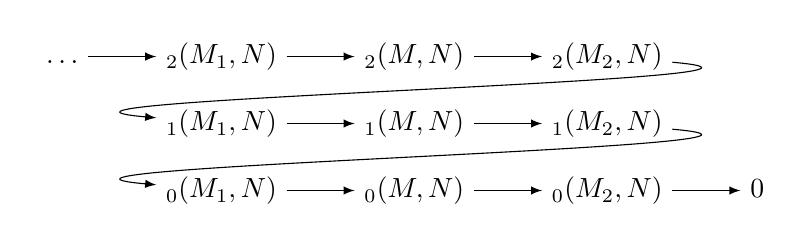
\begin{tikzpicture}
      \matrix (m) [
        matrix of math nodes,
        row sep=1em,
        column sep=2.5em,
        text height=1.5ex, text depth=0.25ex
      ]
      {
        \ldots & \Tor_2(M_1, N) & \Tor_2(M, N) & \Tor_2(M_2, N) &\\
        & \Tor_1(M_1, N) & \Tor_1(M, N) & \Tor_1(M_2, N) &\\
        & \Tor_0(M_1, N) & \Tor_0(M, N) & \Tor_0(M_2, N) & 0\\
      };
      \path[overlay, ->, font=\scriptsize, >=latex]
      (m-1-1) edge (m-1-2)
      (m-1-2) edge (m-1-3)
      (m-1-3) edge (m-1-4)
      (m-1-4) edge[out=355,in=175] (m-2-2)
      (m-2-2) edge (m-2-3)
      (m-2-3) edge (m-2-4)
      (m-2-4) edge[out=355,in=175] (m-3-2)
      (m-3-2) edge (m-3-3)
      (m-3-3) edge (m-3-4)
      (m-3-4) edge (m-3-5);
    \end{tikzpicture}
  \end{center}
  and
  \begin{center}
    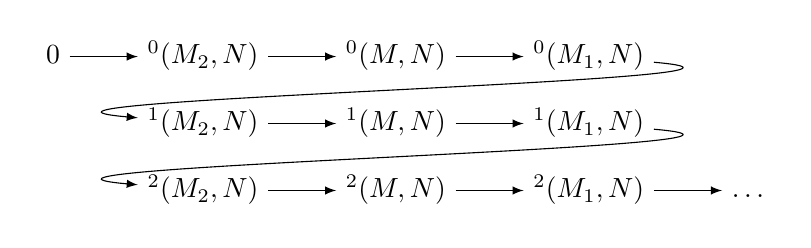
\begin{tikzpicture}
      \matrix (m) [
        matrix of math nodes,
        row sep=1em,
        column sep=2.5em,
        text height=1.5ex, text depth=0.25ex
      ]
      {
        0 & \Ext^0(M_2, N) & \Ext^0(M, N) & \Ext^0(M_1, N) &\\
        & \Ext^1(M_2, N) & \Ext^1(M, N) & \Ext^1(M_1, N) &\\
        & \Ext^2(M_2, N) & \Ext^2(M, N) & \Ext^2(M_1, N) & \ldots\\
      };
      \path[overlay, ->, font=\scriptsize, >=latex]
      (m-1-1) edge (m-1-2)
      (m-1-2) edge (m-1-3)
      (m-1-3) edge (m-1-4)
      (m-1-4) edge[out=355,in=175] (m-2-2)
      (m-2-2) edge (m-2-3)
      (m-2-3) edge (m-2-4)
      (m-2-4) edge[out=355,in=175] (m-3-2)
      (m-3-2) edge (m-3-3)
      (m-3-3) edge (m-3-4)
      (m-3-4) edge (m-3-5);
    \end{tikzpicture}
  \end{center}
\end{theorem}
\begin{corollary}[Dimension Shifting]
  Given a projective presentation $0 \to K \to P \to M \to 0$, one gets
  \[\Tor_n(M,N) = \Tor_{n-1}(K,N); \Ext^n(M,N) = \Ext^{n-1}(K, N)\]
  for $n >0$.
\end{corollary}
\begin{proof}
  Apply \textbf{6.13} to the presentation and note that, for projective $P$, $\Ext^n(P,N) = \Tor_n(P,N) = 0$ for all $n >0$.
\end{proof}
\begin{theorem}[Hilbert's Syzygy Theorem]
  Let $k$ be a field, and $T = k[x_1, \ldots, x_n]$, considered as a graded ring with respect to the total degree of the polynomials. Let $M$ be a finitely generated $T$-module. Then there is a free resolution of $M$ of length $\leq n$.
\end{theorem}
\textbf{Remark.} Example \textbf{6.6} says that the Kosgul complex gives a free resolution of the trivial module of length $n$.
\begin{proof}[Sketch proof.]
  We view $\Tor_n(k, M)$ in two different ways: either
  \begin{itemize}
    \item apply $\cdot \otimes M$ to the Kosgul complex and consider homology groups or
    \item apply $k \otimes \cdot$ to a free resolution of $M$ and consider the homology groups.
  \end{itemize}
  We know that homology groups arising from the two approaches are the same (and $\Tor_n(M,N) = \Tor_n(N,M)$). Write the free resolution as:
  \[\ldots \to F_n \to F_{n-1} \to \ldots \to F_1 \to F_0 \to M \to 0\]
  with each $F_i$ free of finite rank (noetherian). Assume it is also minimal, i.e. with lowest ranks, $\rk(F_0)$ = minimal number of generators - this is called a \emph{minimal free resolution}. Now, if we consider
  \[0 \to K \to F_0 \to M \to 0\]
  where $K$ is the first syzygy module. Then, applying $k \otimes \cdot$, we get a (non-exact) sequence
  \[0 \to k \otimes K \to k \otimes F_0 \to k \otimes M \to 0\]
  Minimality implies that any basis element must be mapped to an element with no constant term in an coefficient, i.e. if $e \in F_{i+1}$ is mapped to $(p_1, \ldots, p_r) \in F_i$, then none of the $p_j$ is constant. This then implies that $k \otimes K \to k \otimes F_0$ is the zero map. Hence the sequence
  \[k \otimes F_n \to k \otimes F_{n-1} \to \ldots \to k \otimes F_0 \to k \otimes M\]
  are all $0$, apart from the last one. Therefore the homology groups are $k \otimes F_i$, which is a finite dimensional $k$-space with dimension equal to the rank of the corresponding free module, apart form the end.

  However, from the description using $\cdot \otimes M$ on the Kosgul complex, we know that $\Tor_i(k, M) = 0$. Thus the free modules $F_i$ in the minimal free resolution for $M$ have rank $0$, and so are $0$, for all $i > n$.
\end{proof}
The text by Zariski/Samuel has a proof without using $\Tor$.
\subsection{Hochschild (Co)homology and Dimension}
This is cohomology theory for bimodules. Let $R$ be a $k$-algebra (not assumed commutative). An $(R,R)$-bimodule is a module where $R$ acts both on the left and on the right, and the two actions commute. We can reformulate in terms of a left or right $(R \otimes_k R^{op})$-module, where $R^{op}$ is defined as the same set as $R$, but with $x \cdot_{R^{op}} y \coloneqq y \cdot_R x$. If $R$ is commutative, then $R^{op} = R$. Then an $(R,R)$-bimodule $M$ is an:
\begin{itemize}
  \item Right $(R\otimes R^{op})$-module, via $r \cdot m \cdot s = m\cdot(s \otimes r)$.
  \item Left $(R \otimes R^{op})$-module, via $r \cdot m \cdot s = (r\otimes s) \cdot m$.
\end{itemize}
\textbf{Examples.}
\begin{itemize}
  \item $R$ is an $(R,R)$-bimodule. This can be extended to $R^n$.
  \item $R \leq S$, then $S$ is an $(R,R)$-bimodule, and also an $(R,S)$ and $(S,R)$-bimodule.
  \item $R \otimes_k R$ is a bimodule, an this extends to $R \otimes \ldots \otimes R$.
  \item We have a bimodule presentation of $R$:
  \[0 \to \ker \mu \to R \otimes R \xrightarrow{\mu} R \to 0\]
  where $\mu(r\otimes s) = rs$. $R \otimes_k R$ is a free bimodule of rank 1, generated by $1 \otimes 1$.
\end{itemize}
\begin{definition}
  Given an $(R,R)$-bimodule $M (= \Tor_n^{R\otimes R^{op}}(R,M)$), the \emph{Hochschild homology} is defined to be
  \[\HH_n(R, M) = \Tor_n^{(R,R)}(R,M)\]
  and the \emph{Hochschild cohomology} is defined to be
  \[\HH^n(R, M) = \Ext_{(R,R)}^n(R,M)\]
\end{definition}
In particular, $\HH^0(R,M) = \Hom_{R,R}(R,M) = \{m \in M: rm = mr \forall r \in R\}$, and $\HH^0(R,R) = Z(R)$, the center of $R$.

Also $\HH_0(R, M) = R \otimes_{(R,R)} M = R \otimes_{R\otimes R^{op}} M = M/\angle{rm-mr: m \in M, r \in R}$.

In particular, $\HH_0(R,R) = R/[R,R]$, where $[r,s] =rs-sr$, the Lie bracket on $R$.

Going back to the last of the examples above, we have $\ker \mu = \angle{r \otimes 1 - 1 \otimes r}$, and if we take a $k$-basis for $R$, then the corresponding elements $r \otimes 1 - 1 \otimes r$ is a $k$-basis for $\ker \mu$.
\begin{definition}
  The \emph{Hoschschild chain complex} gives a free resolution for the bimodule $R$:
  \[\ldots \to R \otimes R \otimes R \xrightarrow{d_0} R \otimes R \xrightarrow{\mu} R \to 0\]
  where $d_{n-1}(r_0 \otimes \ldots \otimes r_{n+1}) = \sum_{i=0}^n (-1)^ij r_0 \otimes \ldots r_i r_{i+1}\otimes \ldots \otimes r_{n+1}$.
\end{definition}
\begin{definition}
  The \emph{Hochschild cohomology dimension} $\Dim R$ of $R$ is
  \[\sup\{n : \HH^n(R, M) \neq 0 \text{ for some bimodule }M\}\]
\end{definition}
\textbf{Remarks.} The $k$-algebras $R$ of $\Dim R = 0$ are precisely those where the bimodule $R$ is projective. This is when $R$ is a direct summand of $R \otimes R$, i.e. $\exists \beta : R \to R \otimes R$ such that $\mu \otimes \beta = \id_R$ ($\mu$ is the above multiplication map). These algebras are called \emph{k-separable}. This generalises the notion of separable field extension. Note that $k$-separable algebras must be finite dimensional as $k$-spaces.
\textbf{Examples.}
\begin{itemize}
  \item $M_n(k)$ is $k$-separable. Given $\beta: R \to R \otimes R$, the image of $1$ is called the \emph{separatory idempotent}. For $M_n(k)$ it is obtained as follows: take $e_{ij}$ to be the elementary matrix with $1$ in the $(i,j)$-entry and $0$ everywhere else. Fix $j$, and consider $\sum_i e_{ij}\otimes e_{ji}$. This is the separatory idempotent. Its image under $\mu$ is $\sum e_ii = 1$, the identity matrix.
  \item Take $\C G$, for $G$ a finite group. Then $\C G \otimes \C G^{op} \cong \C G \otimes \C G \cong \C (G \times G)$, a semisimple algebra. All submodules are direct summands, and in particular $\C G$ is a direct summand of $\C(G \times G)$. Thus $\Dim \C G = 0$.
\end{itemize}
\subsection{Derivations}
$\Hom_{(R,R)}(R \otimes R, M) \cong \Hom_k(k,M)$, as a map is determined by the image of $1 \otimes 1$, since it's free of rank $1$ on this generator. Also,
\[\Hom_{(R,R)}(\underbrace{R\otimes \ldots \otimes R}_{n+2}, M) \cong \Hom_{k}(\underbrace{R \otimes \ldots \otimes R}_{n}, M)\]
\begin{definition}
  The \emph{Hochschild cochain complex} is
  \[M = \Hom_k(k,M) \xrightarrow{\delta_0} \Hom_k(R,M) \xrightarrow{\delta_1} \Hom_k(R\otimes R, M) \to \ldots\]
  where:
  \begin{align*}
    (\delta_0 f)(r) &= rf(1)-f(1)r\\
    (\delta_1 f)(r_1 \otimes r_2) &= r_1f(r_2)-f(r_1r_2)+f(r_1)r_2\\
    (\delta_2 f)(r_1 \otimes r_2 \otimes r_3) &= r_1f(r_2\otimes r_3)-f(r_1r_2\otimes r_3)+f(r_1\otimes r_2r_3) - f(r_1\otimes r_2)r_3
  \end{align*}
  and so on. Then for $\HH^1(R,M)$, we want $\ker \delta_1/\im \delta_0$.
\end{definition}
\begin{definition}
  $\ker \delta_1 = \{f \in \Hom_k(R,M) : f(r_1r_2) = r_1f(r_2) + f(r_1)r_2\}$ is the set of \emph{derivations} $R \to M$, written $\Der(R,M)$.
  \[\im \delta_0 = \{f \in \Hom_k(R,M) : f\text{ of the form }r\mapsto rm-mr\text{ for some m}\}\]
  are the \emph{inner derivations}, written $\Inn\Der(R,M)$. So
  \[\HH^1(R,M) = \Der(R,M)/\Inn\Der(R,M)\]
\end{definition}
\textbf{Examples.}
\begin{itemize}
  \item $M=R$: $\HH^1(R,R) = \Der(R)/\Inn\Der(R)$.
  \item If $R$ is commutative, $\Inn\Der(R) = 0$, and so $\HH^1(R,R) = \Der(R)$.
  \item In general, $\Der(R)$ forms a Lie algebra. If $D_1, D_2$ are derivations $R \to R$, then $D_1 D_2 - D_2 D_1 \in \End_k(R)$ is also a derivation.
  \item If $\theta \in \Hom_{(R,R)}(R\otimes_k R, M)$, it is determined by the image $m$ of $1 \otimes 1$, and the restriction to $\ker \mu$ is the map $r \otimes 1 - 1 \otimes r \mapsto rm-mr$.

  Consider $\phi \in \Hom_{(R,R)}(\ker \mu, M)$. Define $d : R \to M; r \mapsto \psi(r\otimes 1 -1 \otimes r)$.

  Note that $rs \mapsto \phi(rs \otimes 1-1 \otimes rs) = \phi(r(s\otimes 1-1\otimes s)+(r\otimes 1-1\otimes r)s) = rd(s)+d(r)s.$
  \item $R = k[x]$. $\Der(R) = \{p(x)\frac{d}{dx} : p(x) \in k[x]\}$, where $\charr k = 0$ (otherwise differentiation doesn't behave well).
  \item In the case $M=R$, an $(R,R)$-bimodule when $R$ is commutative, we have that derivations are examples of differential operators: if $R$ is a commutative $k$-algebra, we define differential operators iteratively as:
  \[D(R) = \bigcup D^i(R): D^0(R) = \{D \in \End(R):[r,D] = 0 \forall r \in R\}\]
  and then
  \[D^i(R) = \{D \in \End(R):[r,D]\in D^{i-1}(R) \forall r \in R\}\]
  \item For example, $D(k[x]) = k[x, \frac{d}{dx}] \subseteq \End_k(k[x])$. If $R = k[x_1, \ldots, x_n]$ and $\charr k = 0$, then, by induction
  \[D(k[x_1, \ldots, x_n]) = k[x_1, \frac{\partial}{\partial x_1}, \ldots, x_n, \frac{\partial}{\partial x_n}]\]
\end{itemize}
\begin{definition}
  Given $M$ an $(R,R)$-bimodule, we form the \emph{semidirect product} $R \ltimes M$ with addition as usual, but multiplication given by $(r_1, m_1)\cdot (r_2, m_2) = (r_1r_1, r_1m_2+m_1r_2)$. Alternatively, this is $R+ M\epsilon$ where $\epsilon^2 =0$, and $\epsilon$ commutes with everything. $M \epsilon$ is an ideal and $(M\epsilon)^2 = 0$.
\end{definition}
\begin{lemma}
  $\Der(R,M) \cong \{\text{algebra complement to }M \text{ in }R \ltimes M\}$.
\end{lemma}
\begin{proof}
  A complement to $M$ is an embedded copy of $R$ in $R\ltimes M$:
  \[R \injection R \ltimes M; r \mapsto (r, D(r))\]
  This function $D: R \to M$ is a derivation. Conversely, $D: R \to M$ gives such an embedding.
\end{proof}
\begin{corollary}
  $\Der(R,M) = \{\text{automorphisms of }R \ltimes M = R+M\epsilon\}$, where on $R \ltimes M, r\mapsto (r, D(r))$ and $m \mapsto m$ corresponds to on $R+M\epsilon$, $r\mapsto r+D(r)\epsilon, m\epsilon \mapsto m\epsilon$. $\Inn\Der(R,M) = \{\text{automorphisms of }R \ltimes M \text{ of the form obtained by conjugation by }1+m\epsilon\}$.
\end{corollary}
\end{document}
